
\chapter{Web-based QPJ-BR questionnaire}
\label{annex:QPJ-BR-questionnaire}
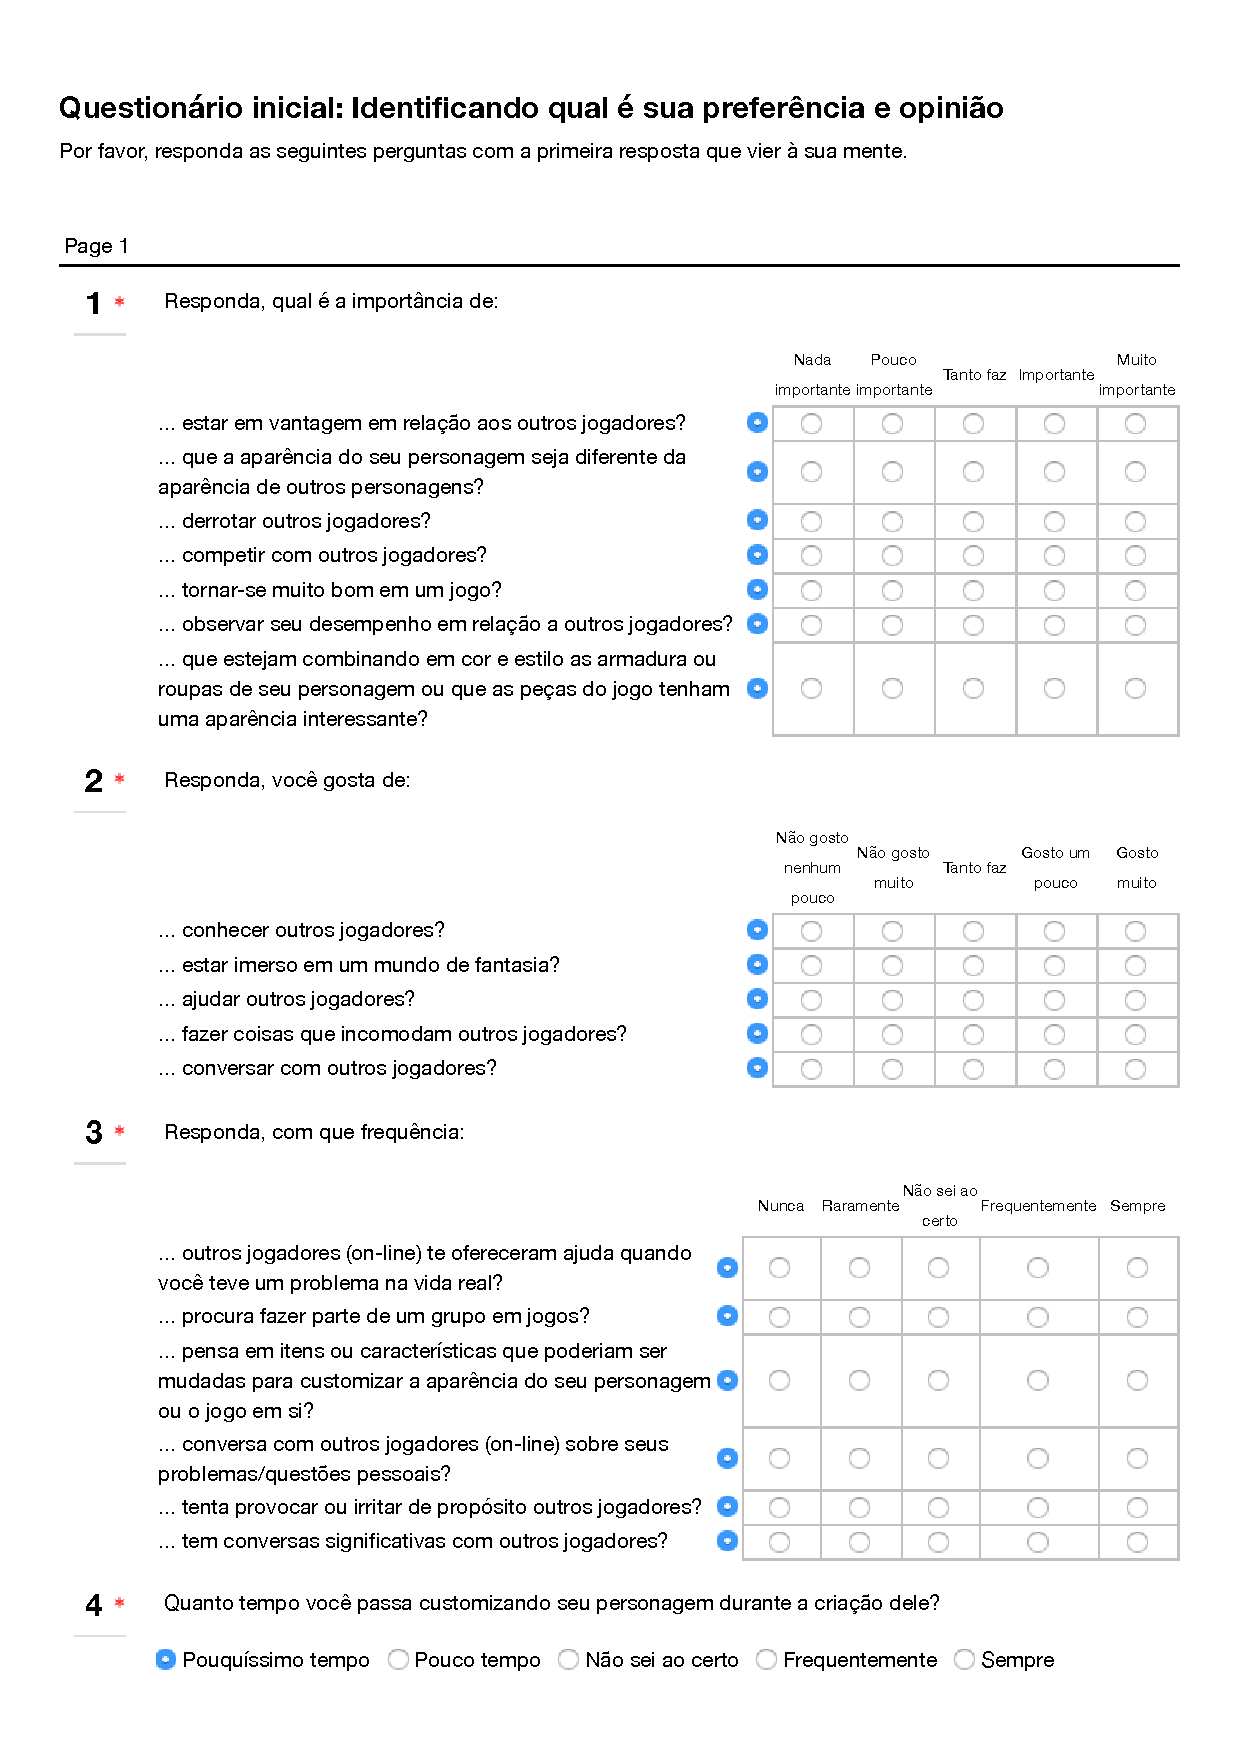
\includegraphics[page=1,width=1\textwidth]{images/annex/QPJ-BR-questionnaire.pdf}

%% ========== %%
\chapter{Data Gathering Instruments for Measuring Participants' Skill and Knowledge}
\label{annex:data-gathering-instruments-skill-knowledge}

\section{Programming Problem: Calculate the Proper Divisors of a Number (P1')}
\label{annex:pilot-study-p1}
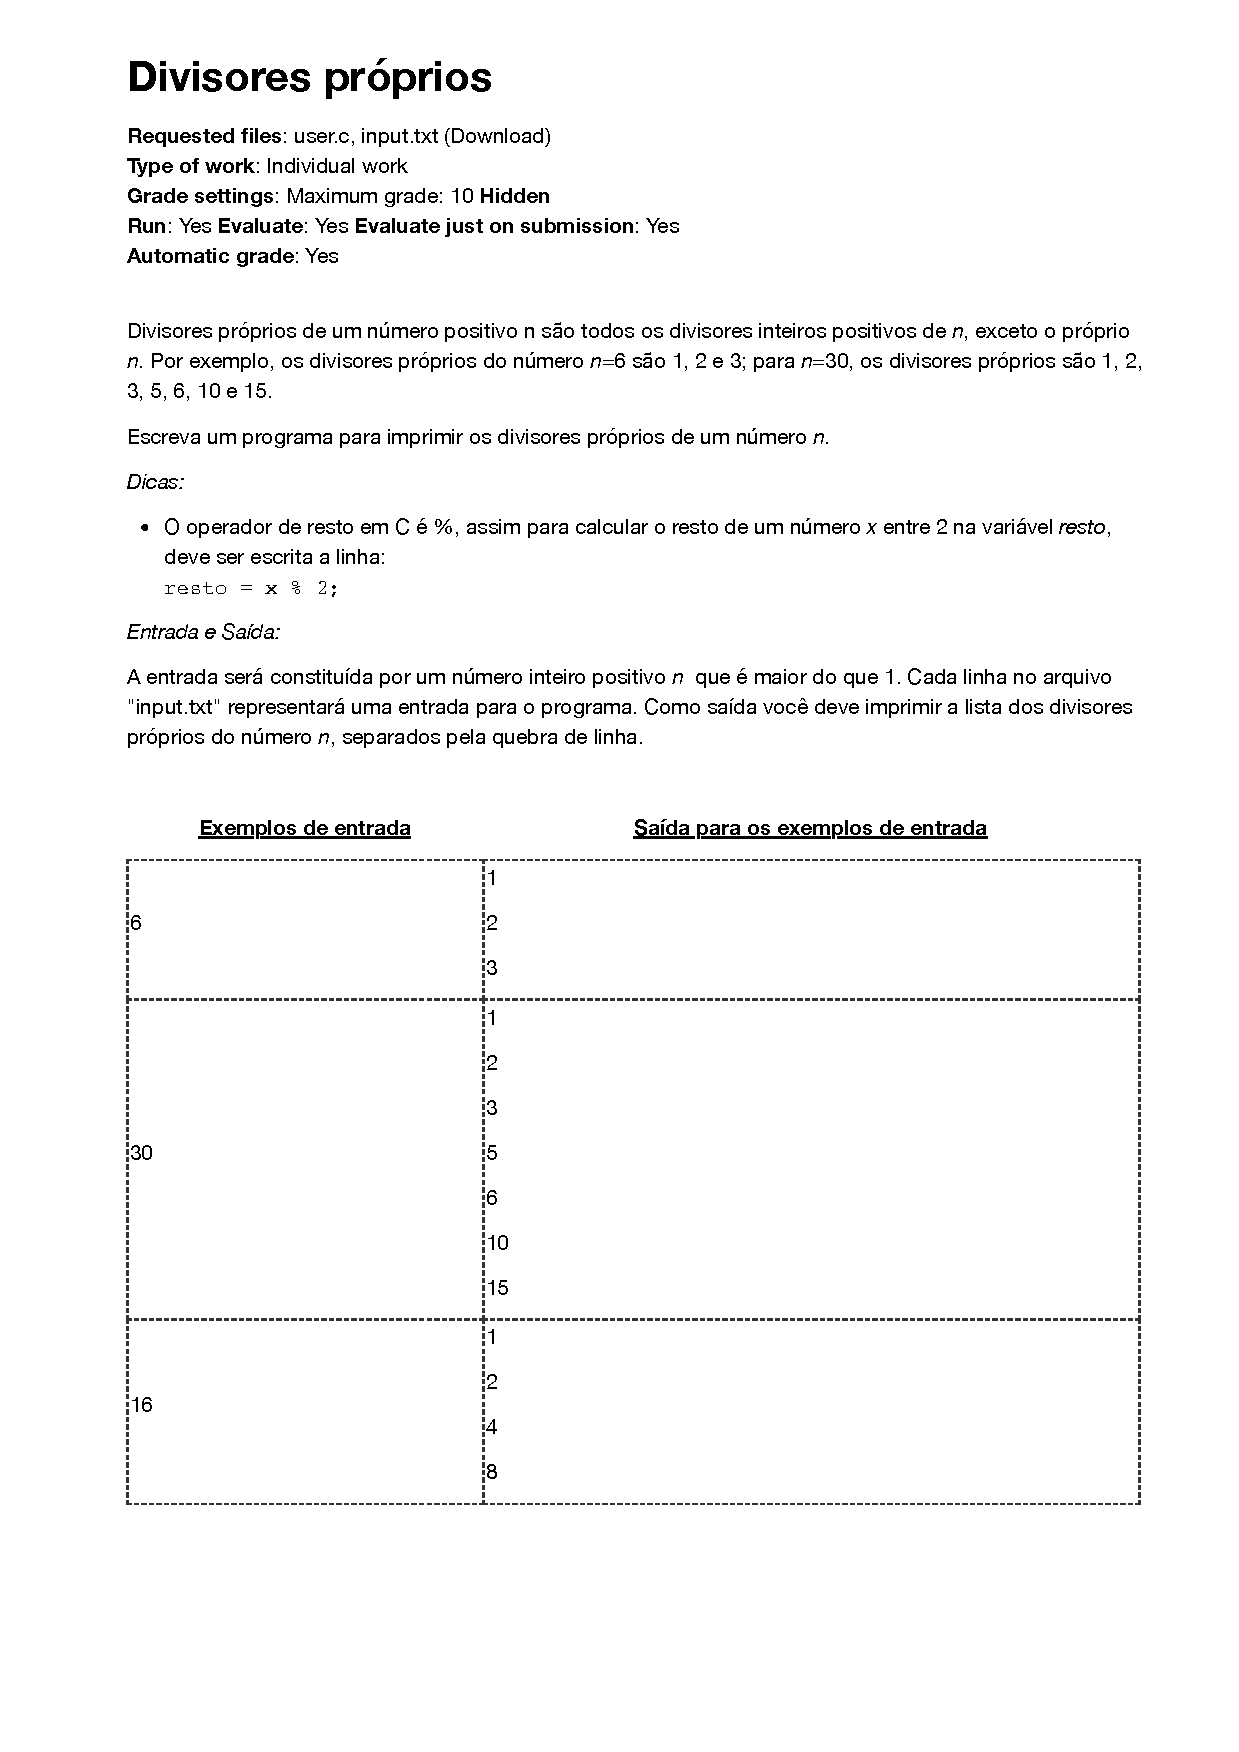
\includegraphics[page=1,width=1\textwidth]{images/annex/pilot-study-p1.pdf}

\newpage
\section{Programming Problem: Calculate the Sum of Prime Divisors of Number (P2')}
\label{annex:pilot-study-p2}
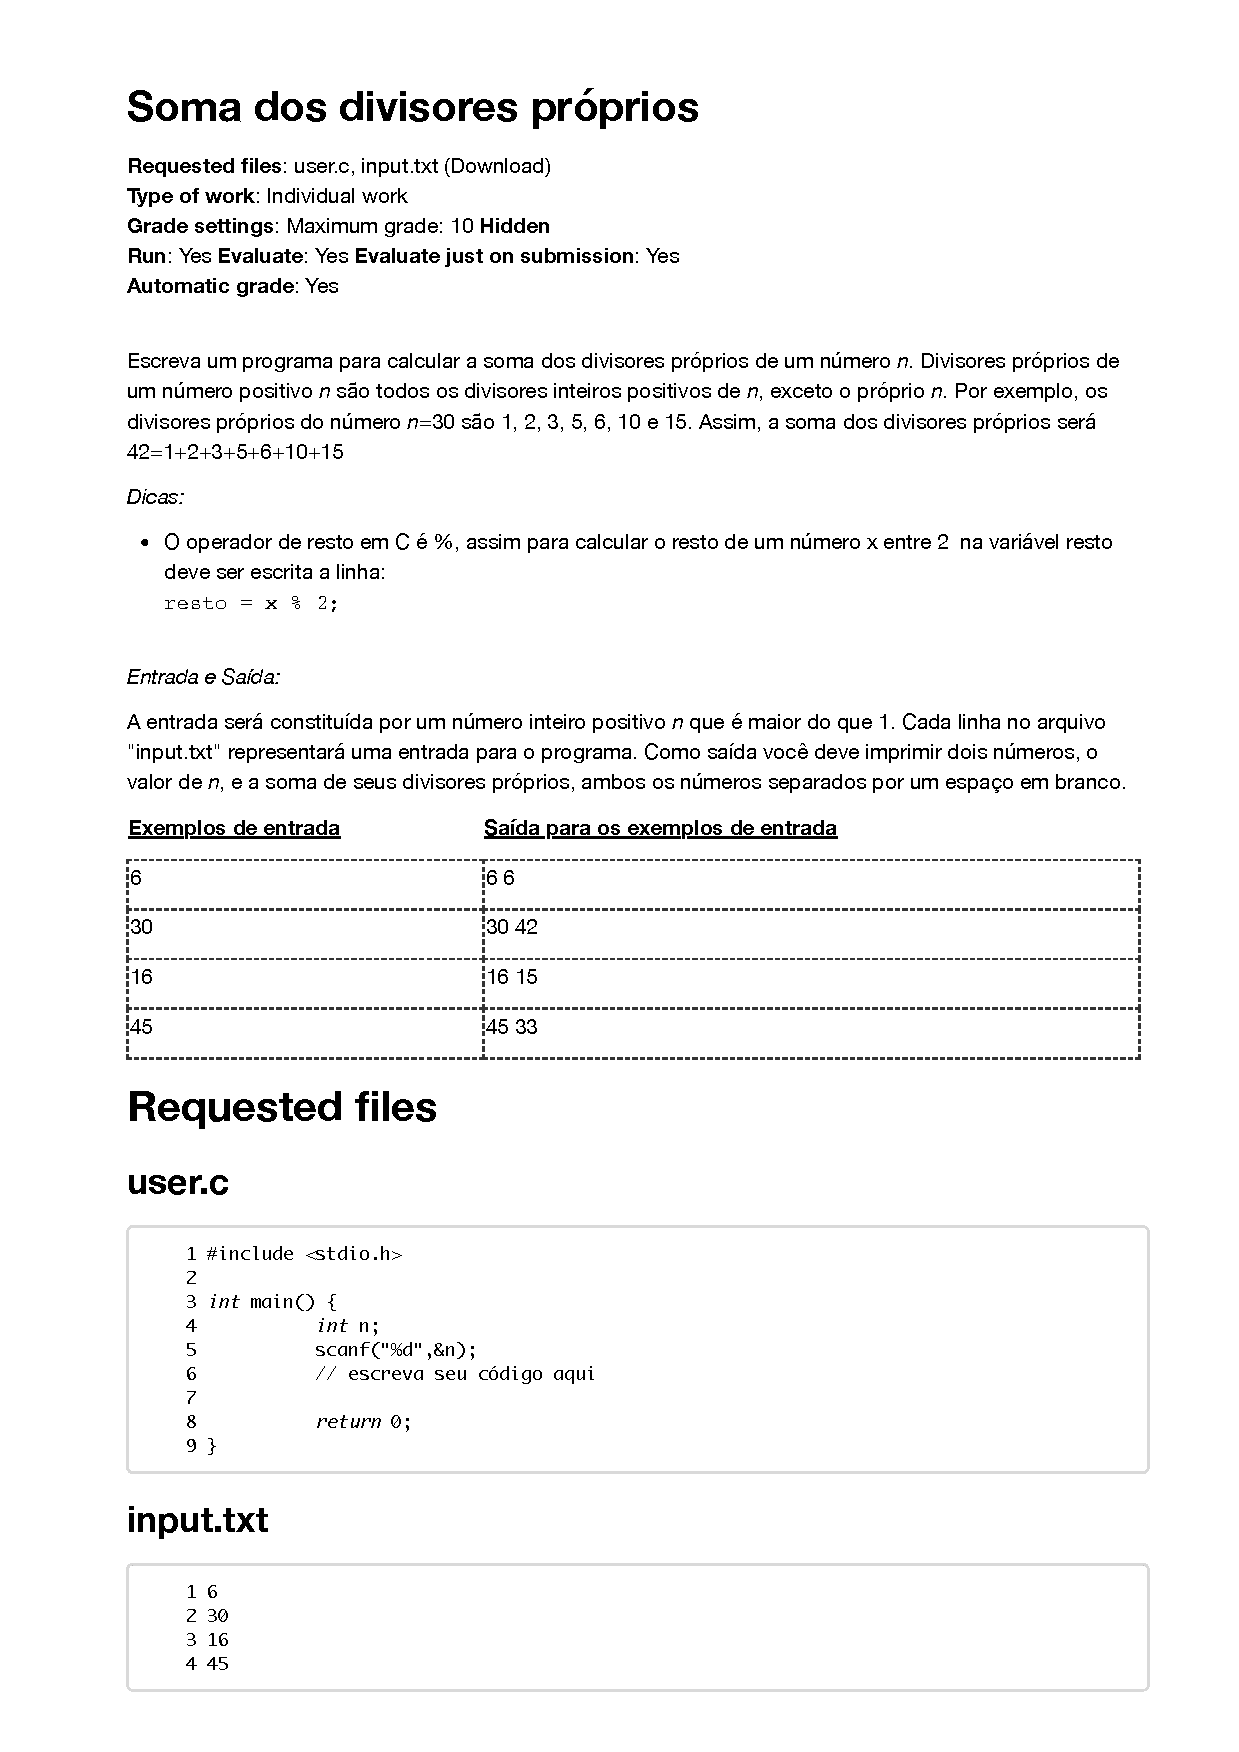
\includegraphics[page=1,width=1\textwidth]{images/annex/pilot-study-p2.pdf}

\newpage
\section{Programming Problem: Calculate Distance of Rebounds for an Elastic Ball (P3')}
\label{annex:pilot-study-p3}
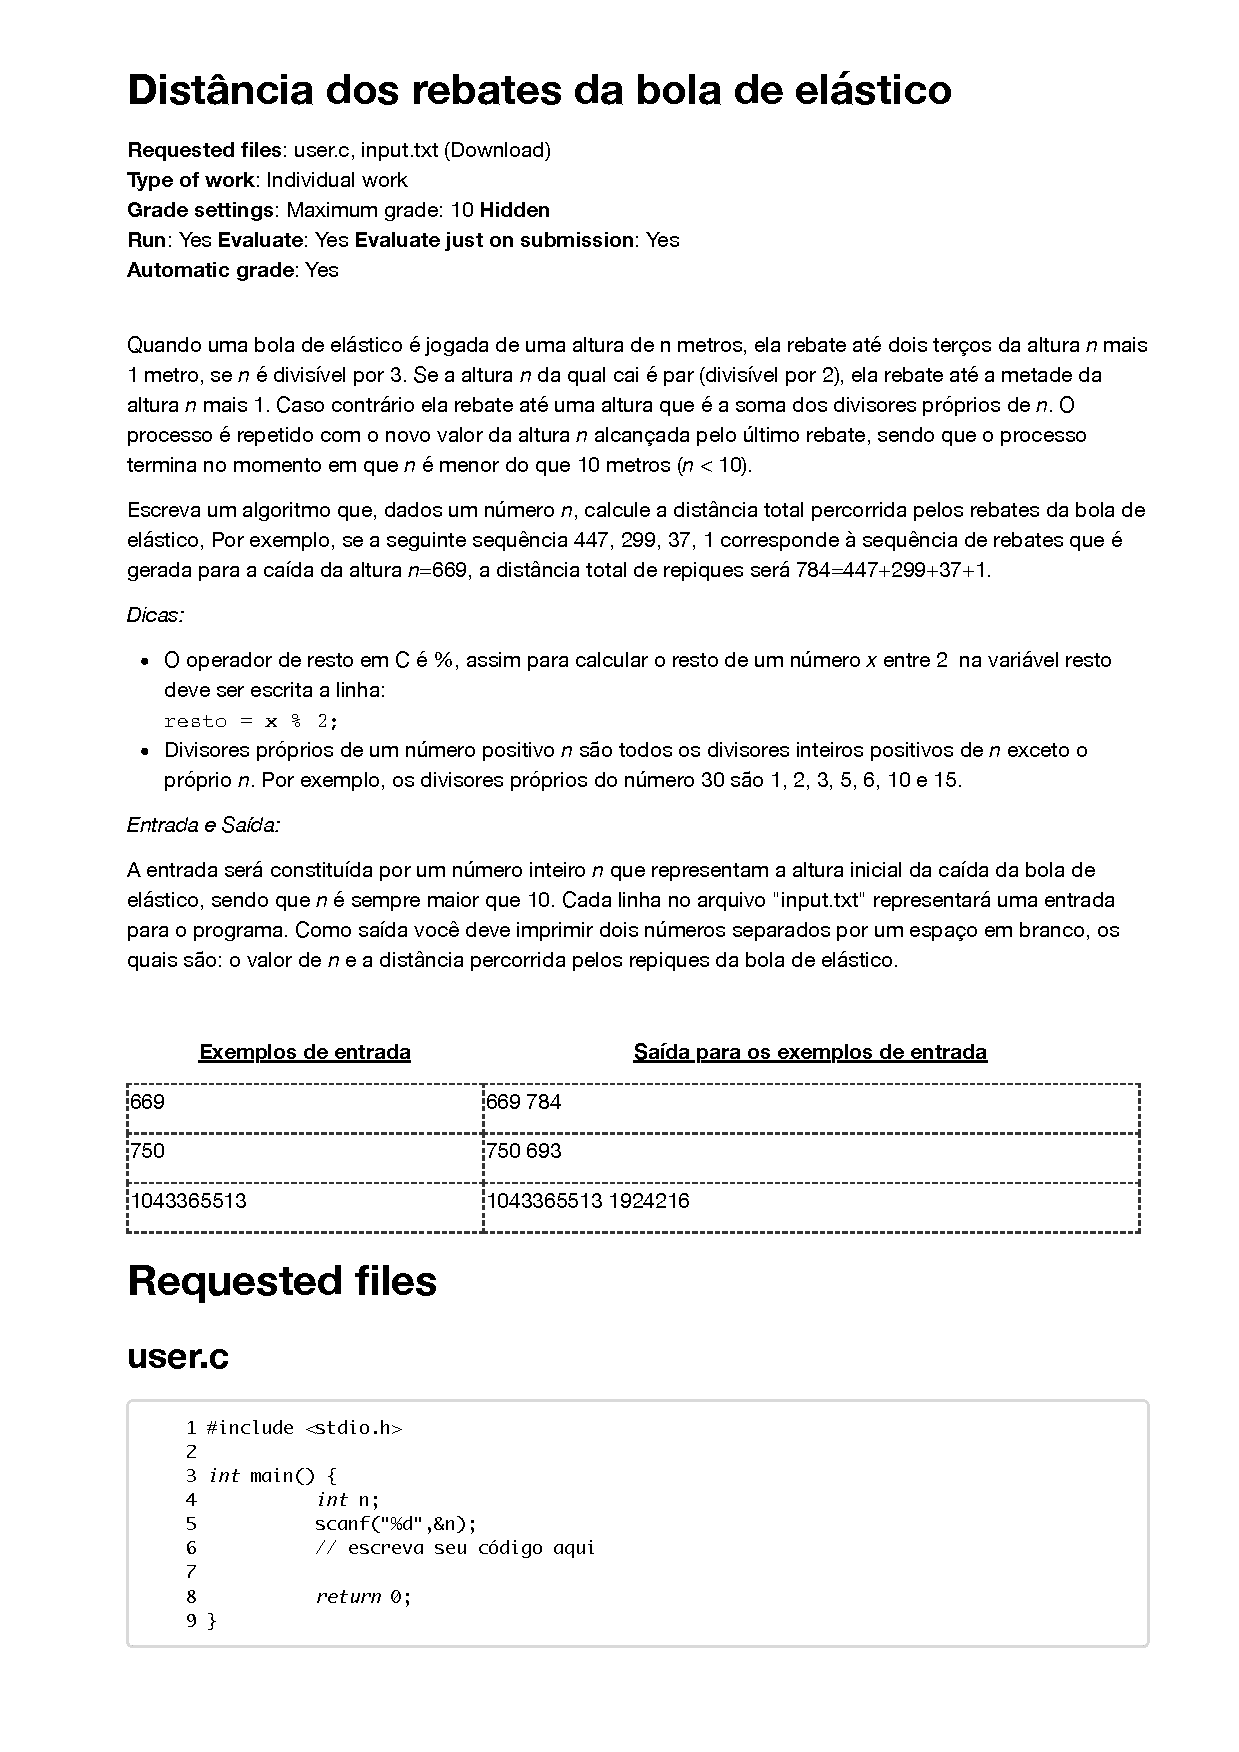
\includegraphics[page=1,width=1\textwidth]{images/annex/pilot-study-p3.pdf}

\newpage
\section{Programming Problem: Calculate the Maximum Length of a Hailstone Sequence (P4')}
\label{annex:pilot-study-p4}

\includegraphics[page=1,width=1\textwidth]{images/annex/pilot-study-p4.pdf}

\newpage
\section{Programming Problem: Calculate Inverse Fibonacci Sequence on Base $n$ and $m$ (PA')}
\label{annex:pilot-study-pA}
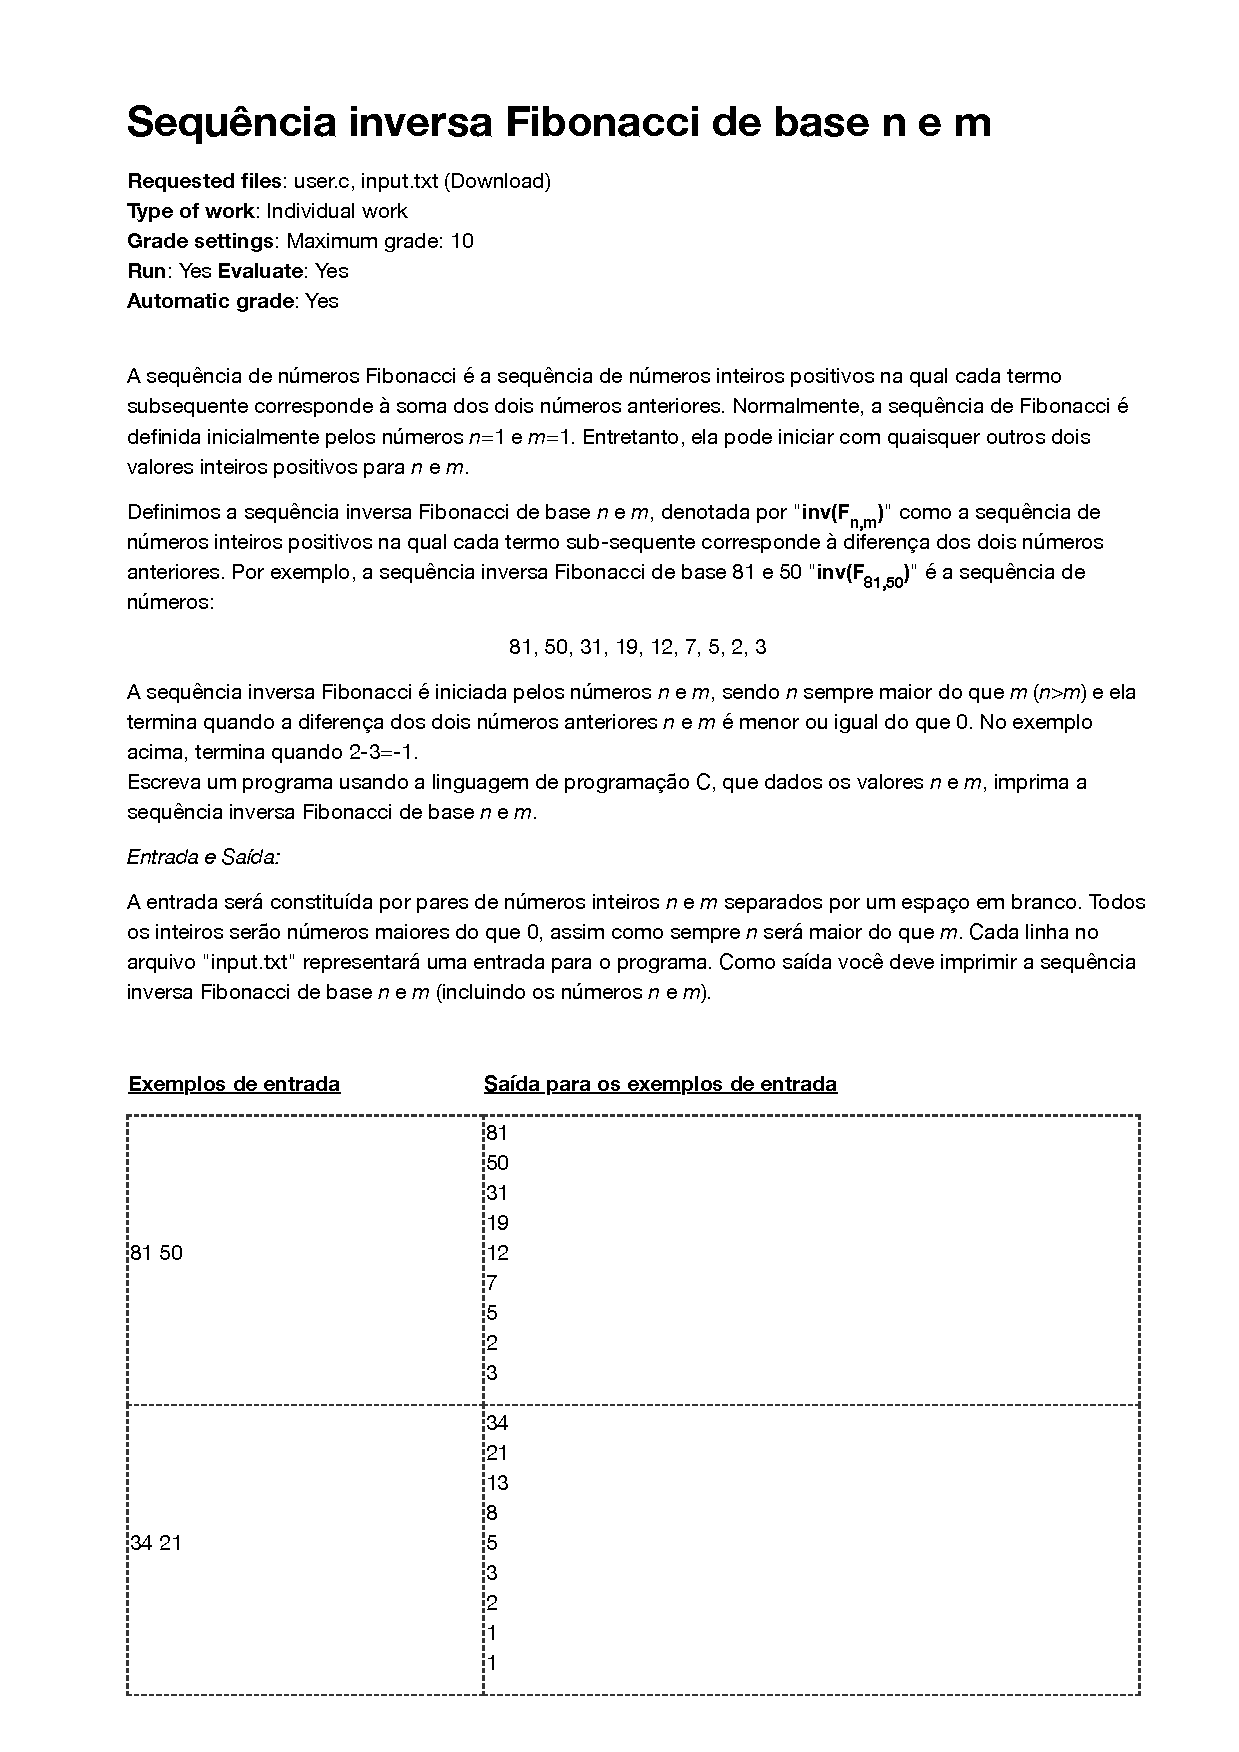
\includegraphics[page=1,width=1\textwidth]{images/annex/pilot-study-pA.pdf}


\newpage
\section{Programming Problem: Calculate the Absolute Difference Between Odd and Even Numbers in an Inverse Fibonacci Sequence (PB')}
\label{annex:pilot-study-pB}
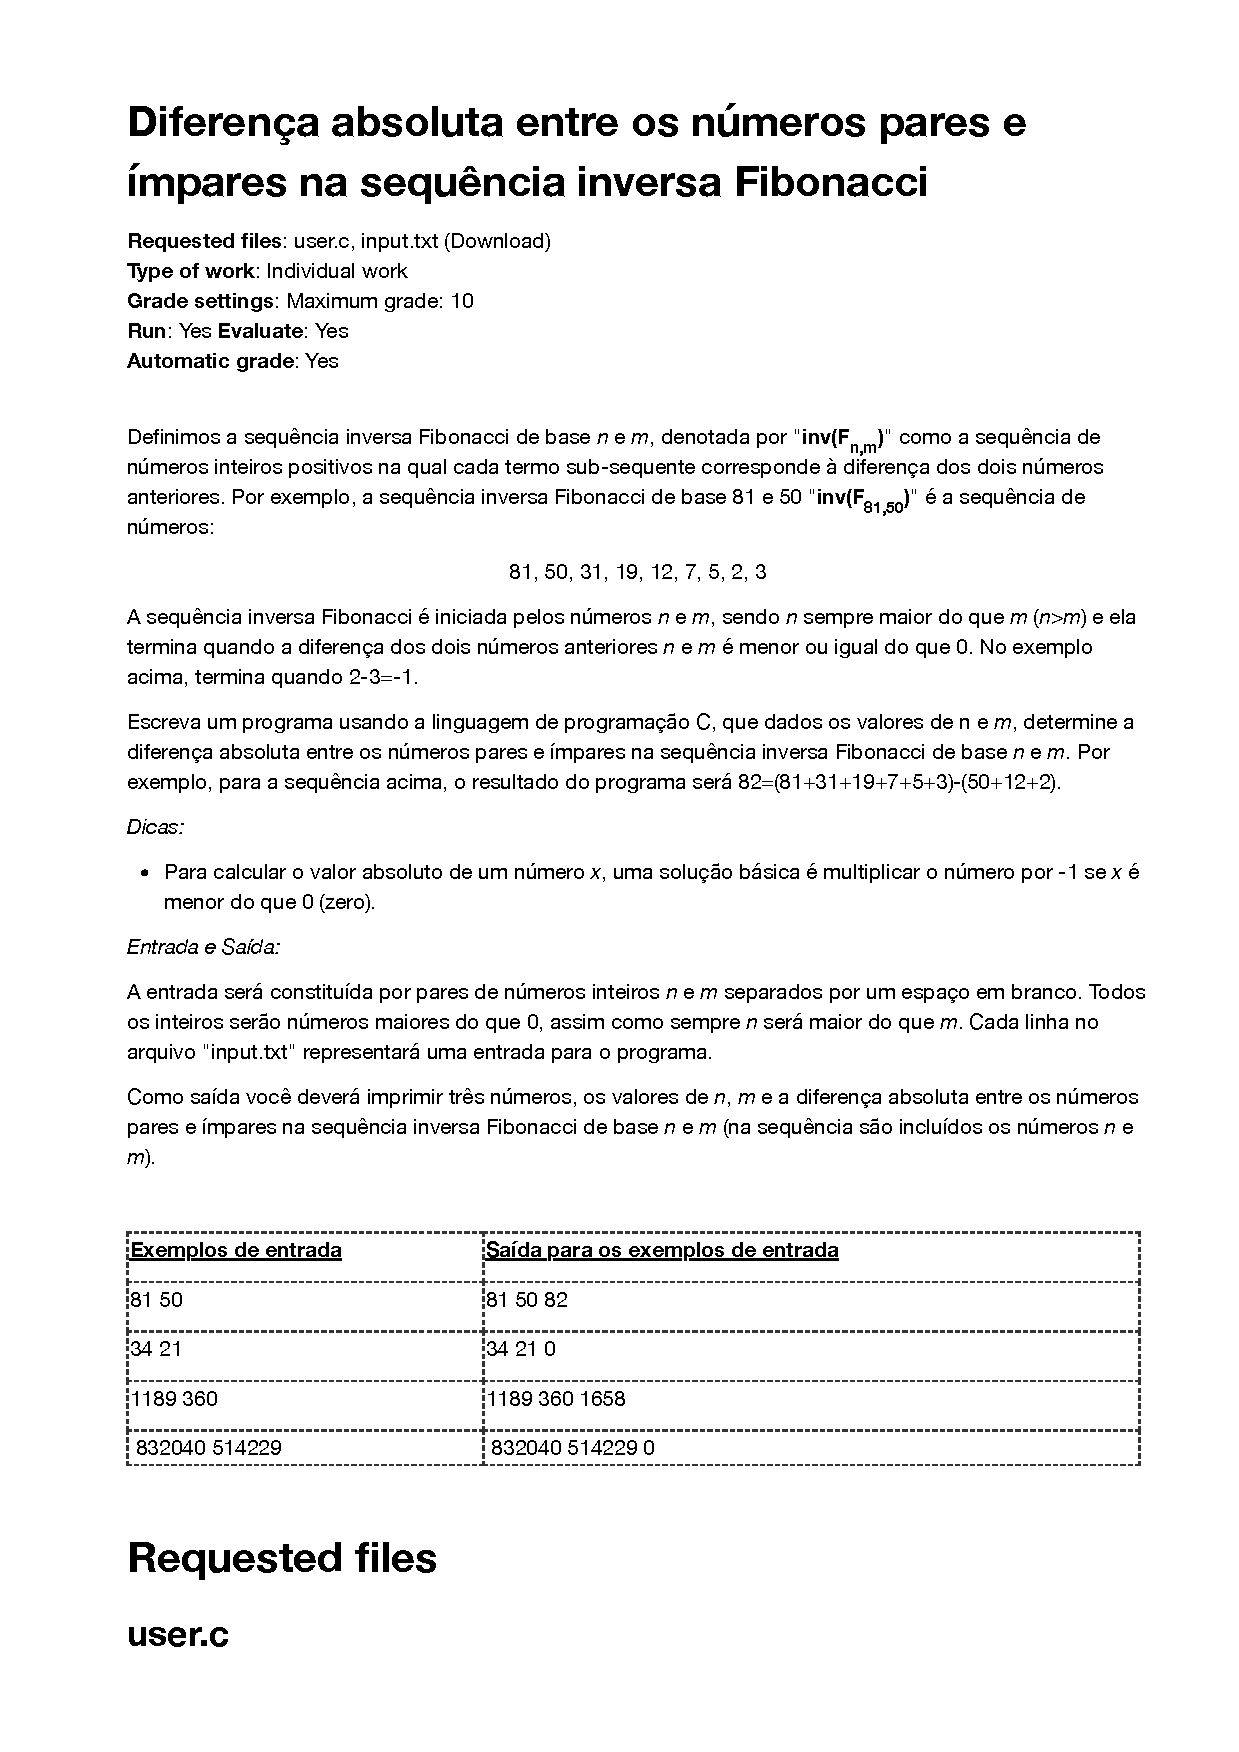
\includegraphics[page=1,width=1\textwidth]{images/annex/pilot-study-pB.pdf}

\newpage
\section{Programming Problem: Calculate the i-th Prize of a Machine Slot (PC')}
\label{annex:pilot-study-pC}
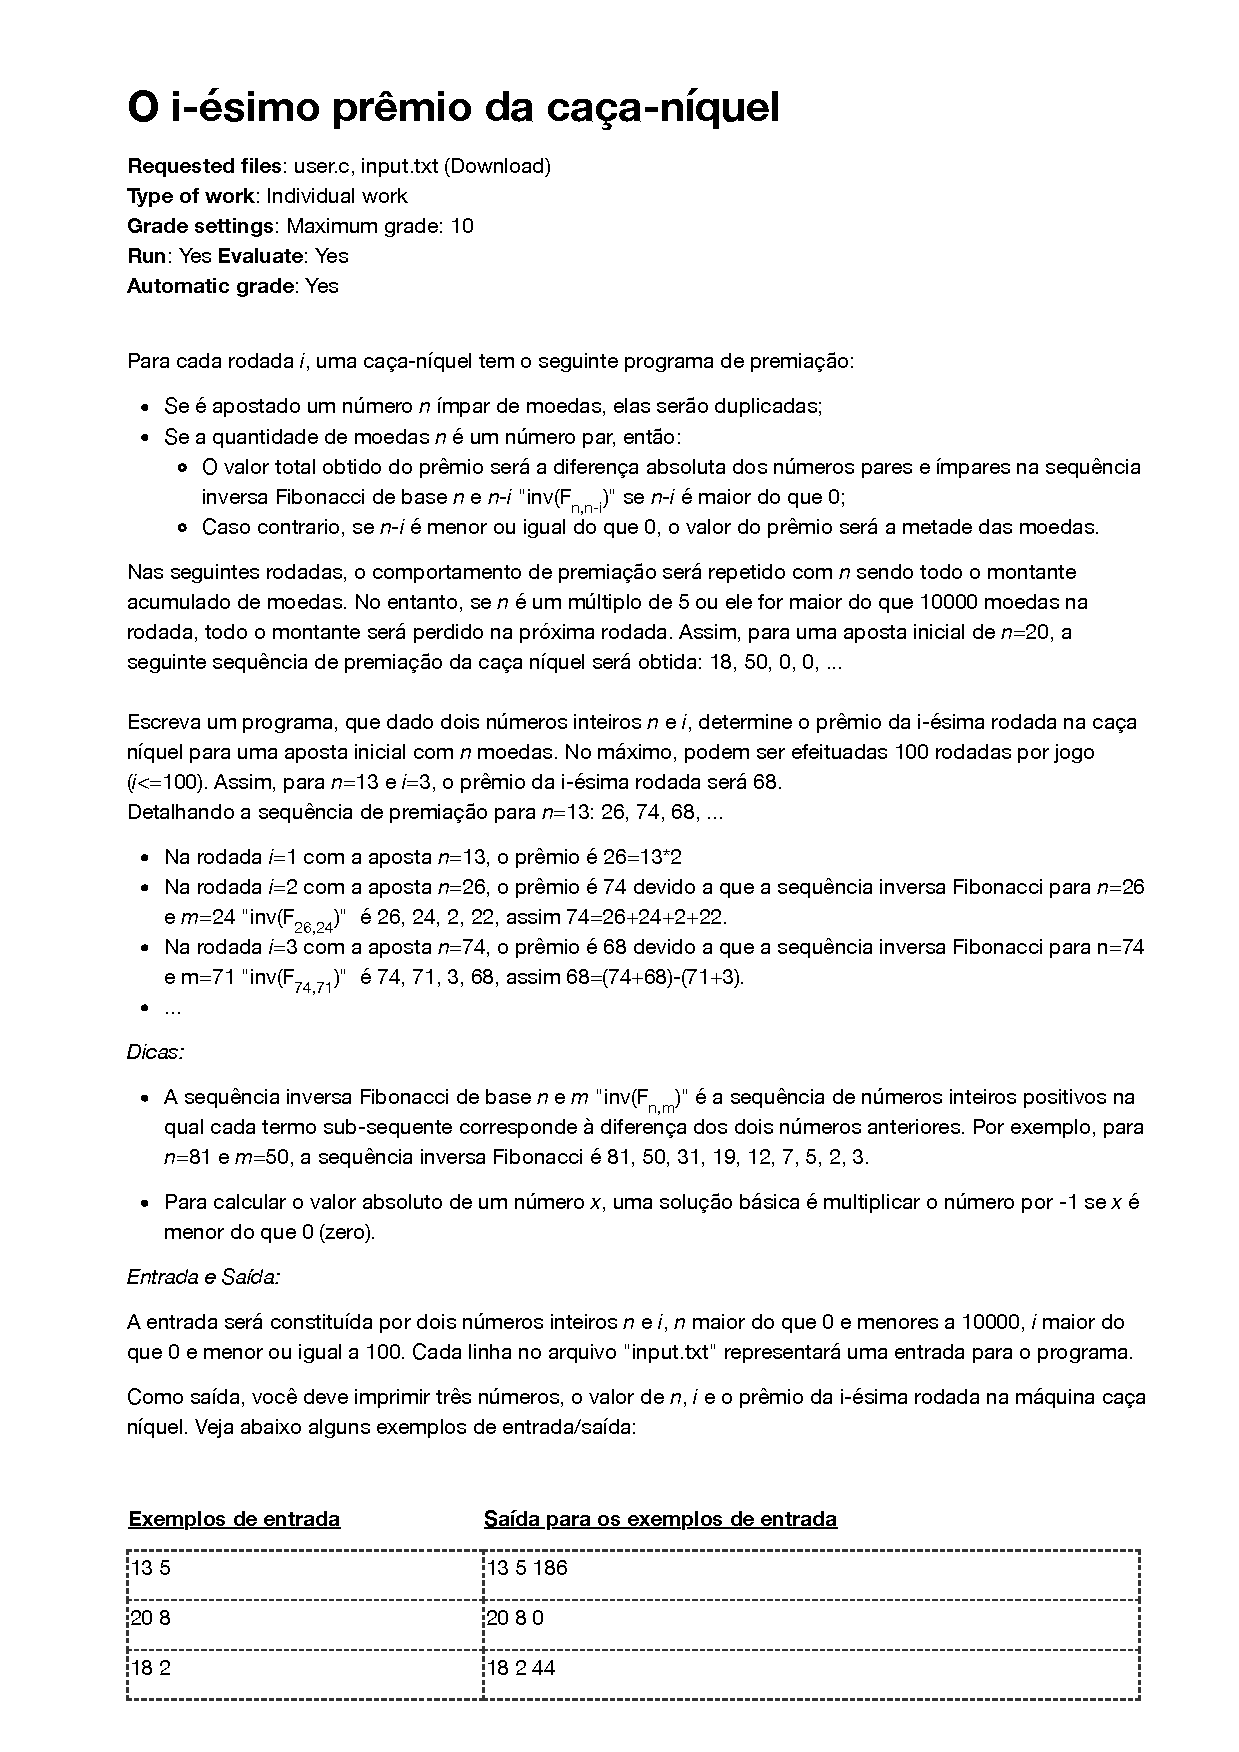
\includegraphics[page=1,width=1\textwidth]{images/annex/pilot-study-pC.pdf}

\newpage
\section{Programming Problem: Calculate the Highest Prize of a Machine Slot (PD')}
\label{annex:pilot-study-pD}
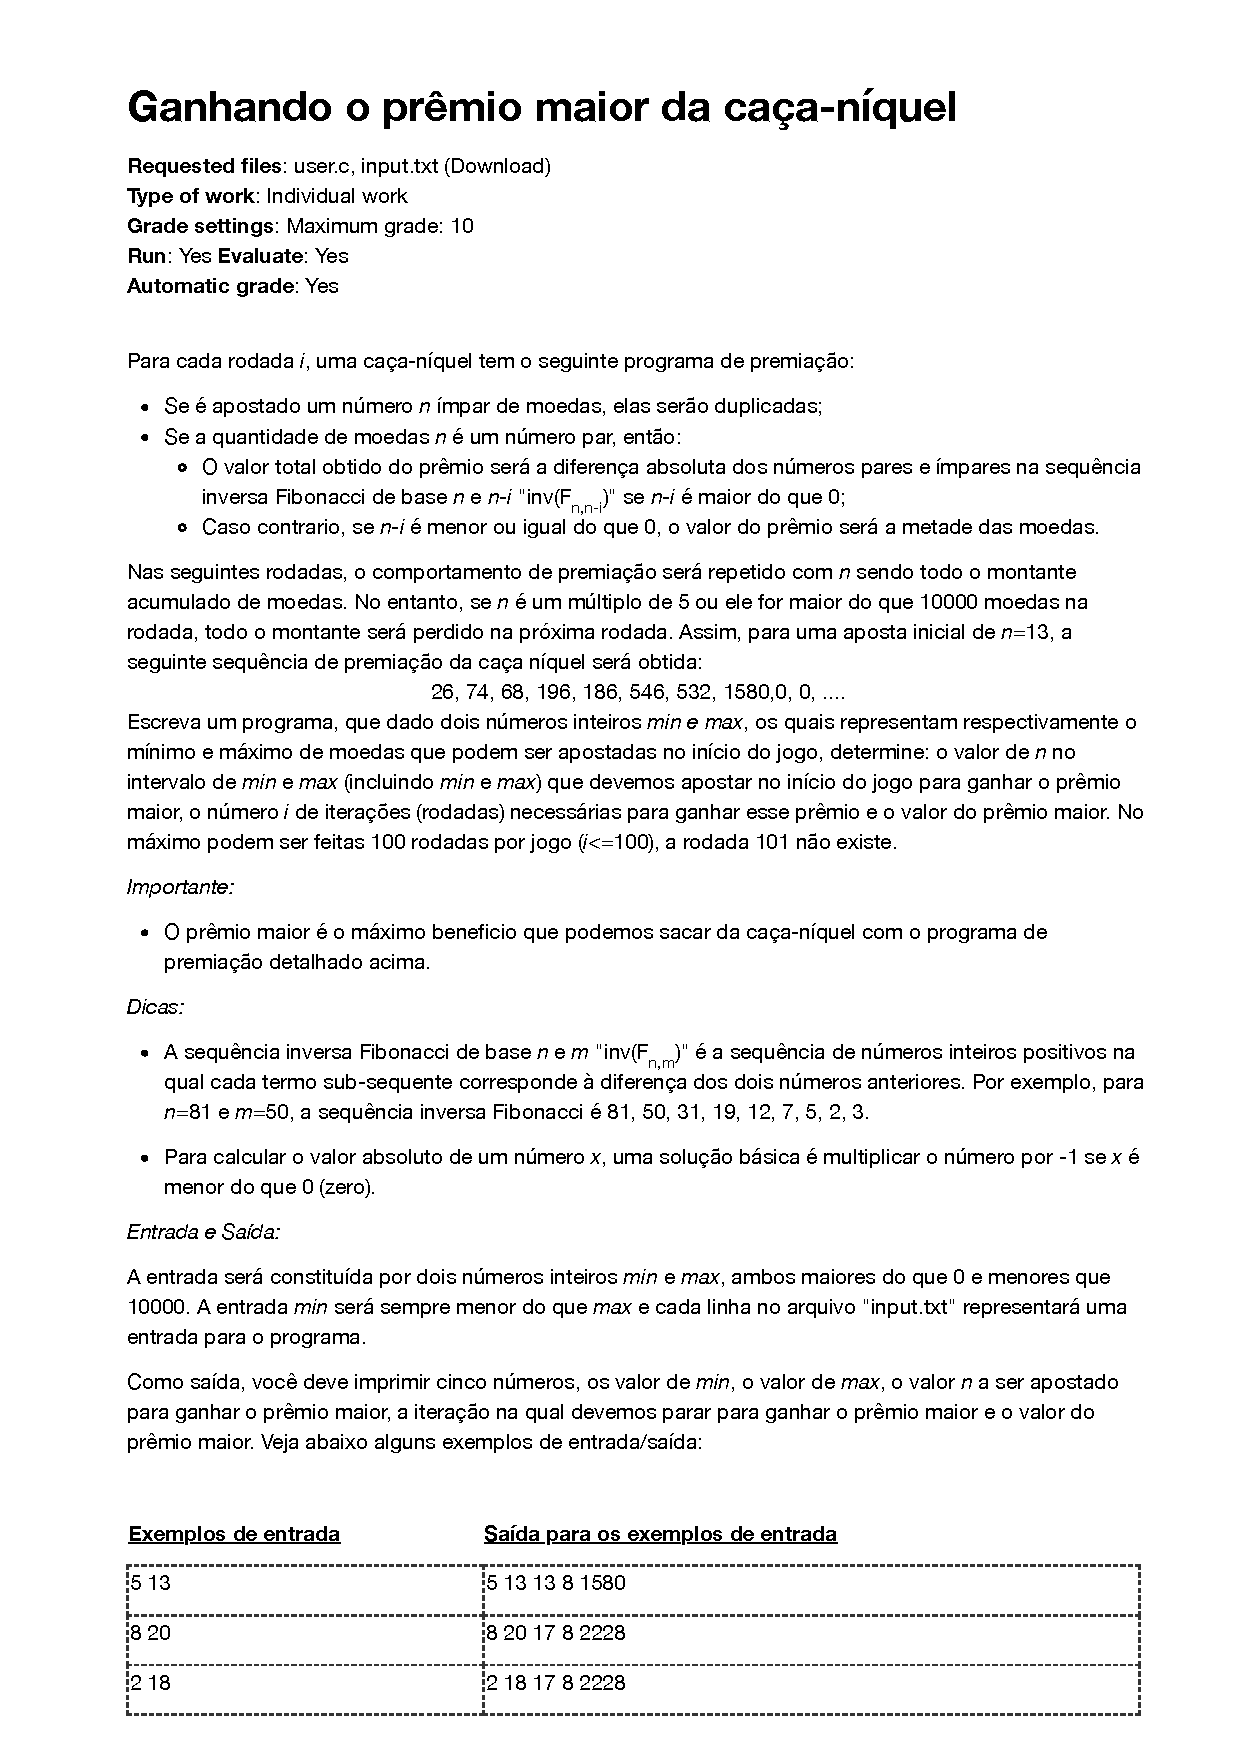
\includegraphics[page=1,width=1\textwidth]{images/annex/pilot-study-pD.pdf}

\newpage
\section{Formative Evaluation: Multiple Choice Knowledge Questionnaires of Cond. Structures (provinha1a)}
\label{annex:first-study-pre}
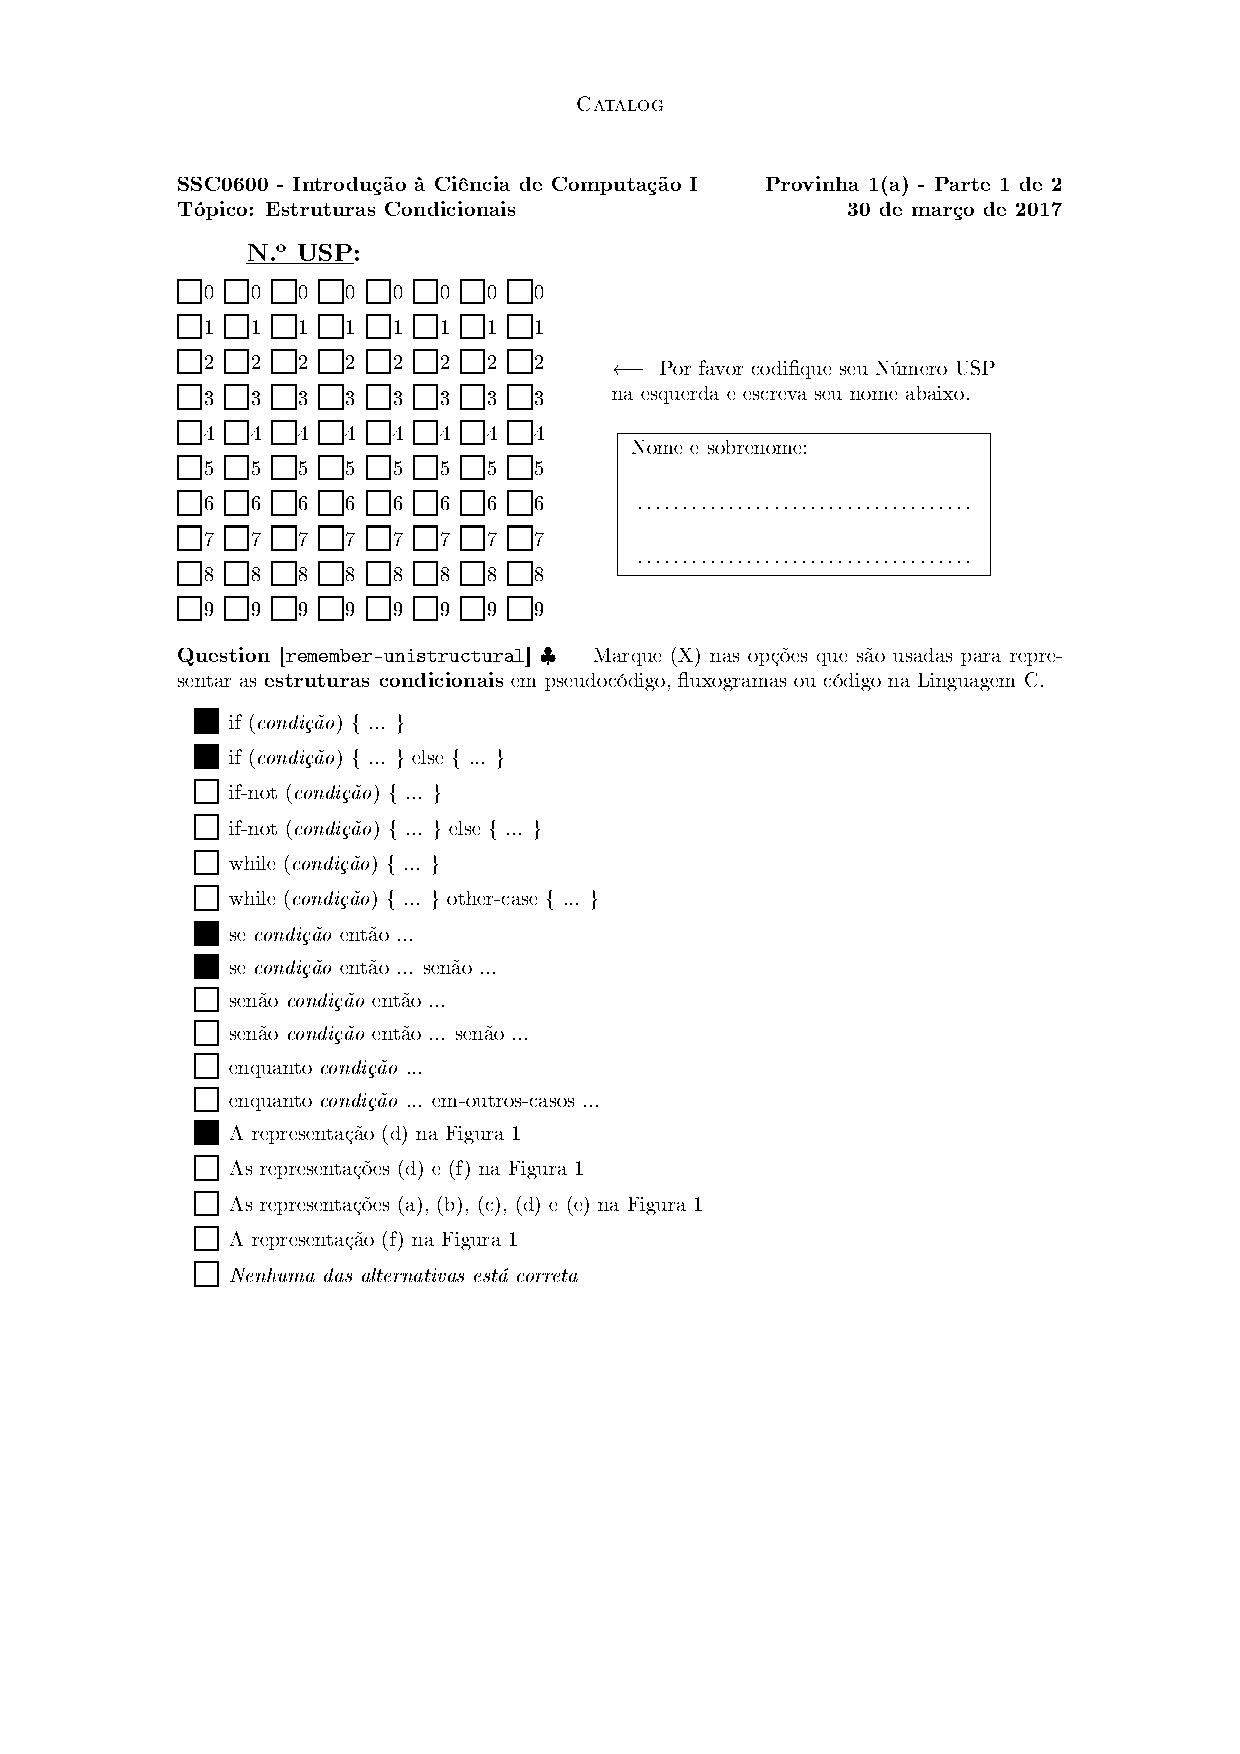
\includegraphics[page=1,width=1\textwidth]{images/annex/first-study-pre-1.pdf}
\newpage
\includegraphics[page=2,width=1\textwidth]{images/annex/first-study-pre-1.pdf}
\newpage
\includegraphics[page=3,width=1\textwidth]{images/annex/first-study-pre-1.pdf}
\newpage
\includegraphics[page=4,width=1\textwidth]{images/annex/first-study-pre-1.pdf}
\newpage
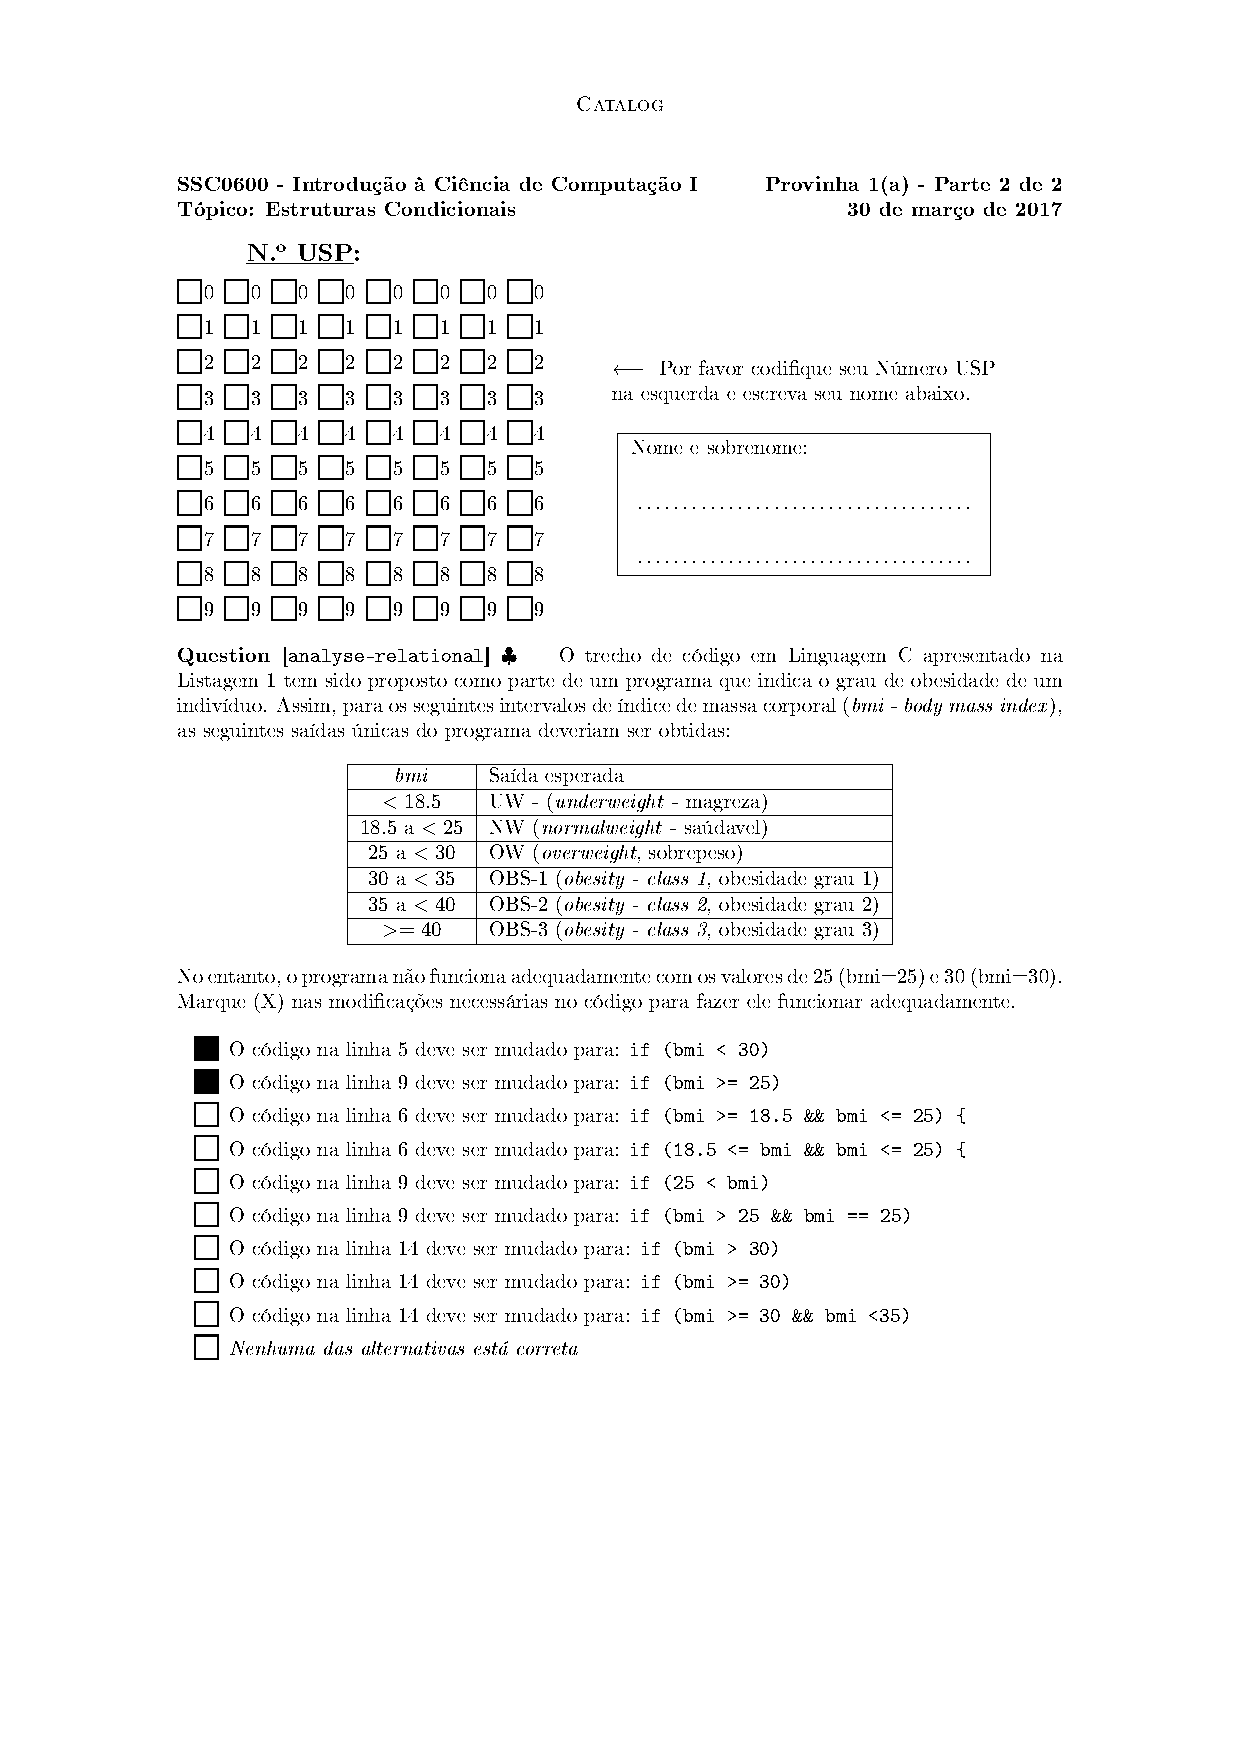
\includegraphics[page=1,width=1\textwidth]{images/annex/first-study-pre-2.pdf}
\newpage
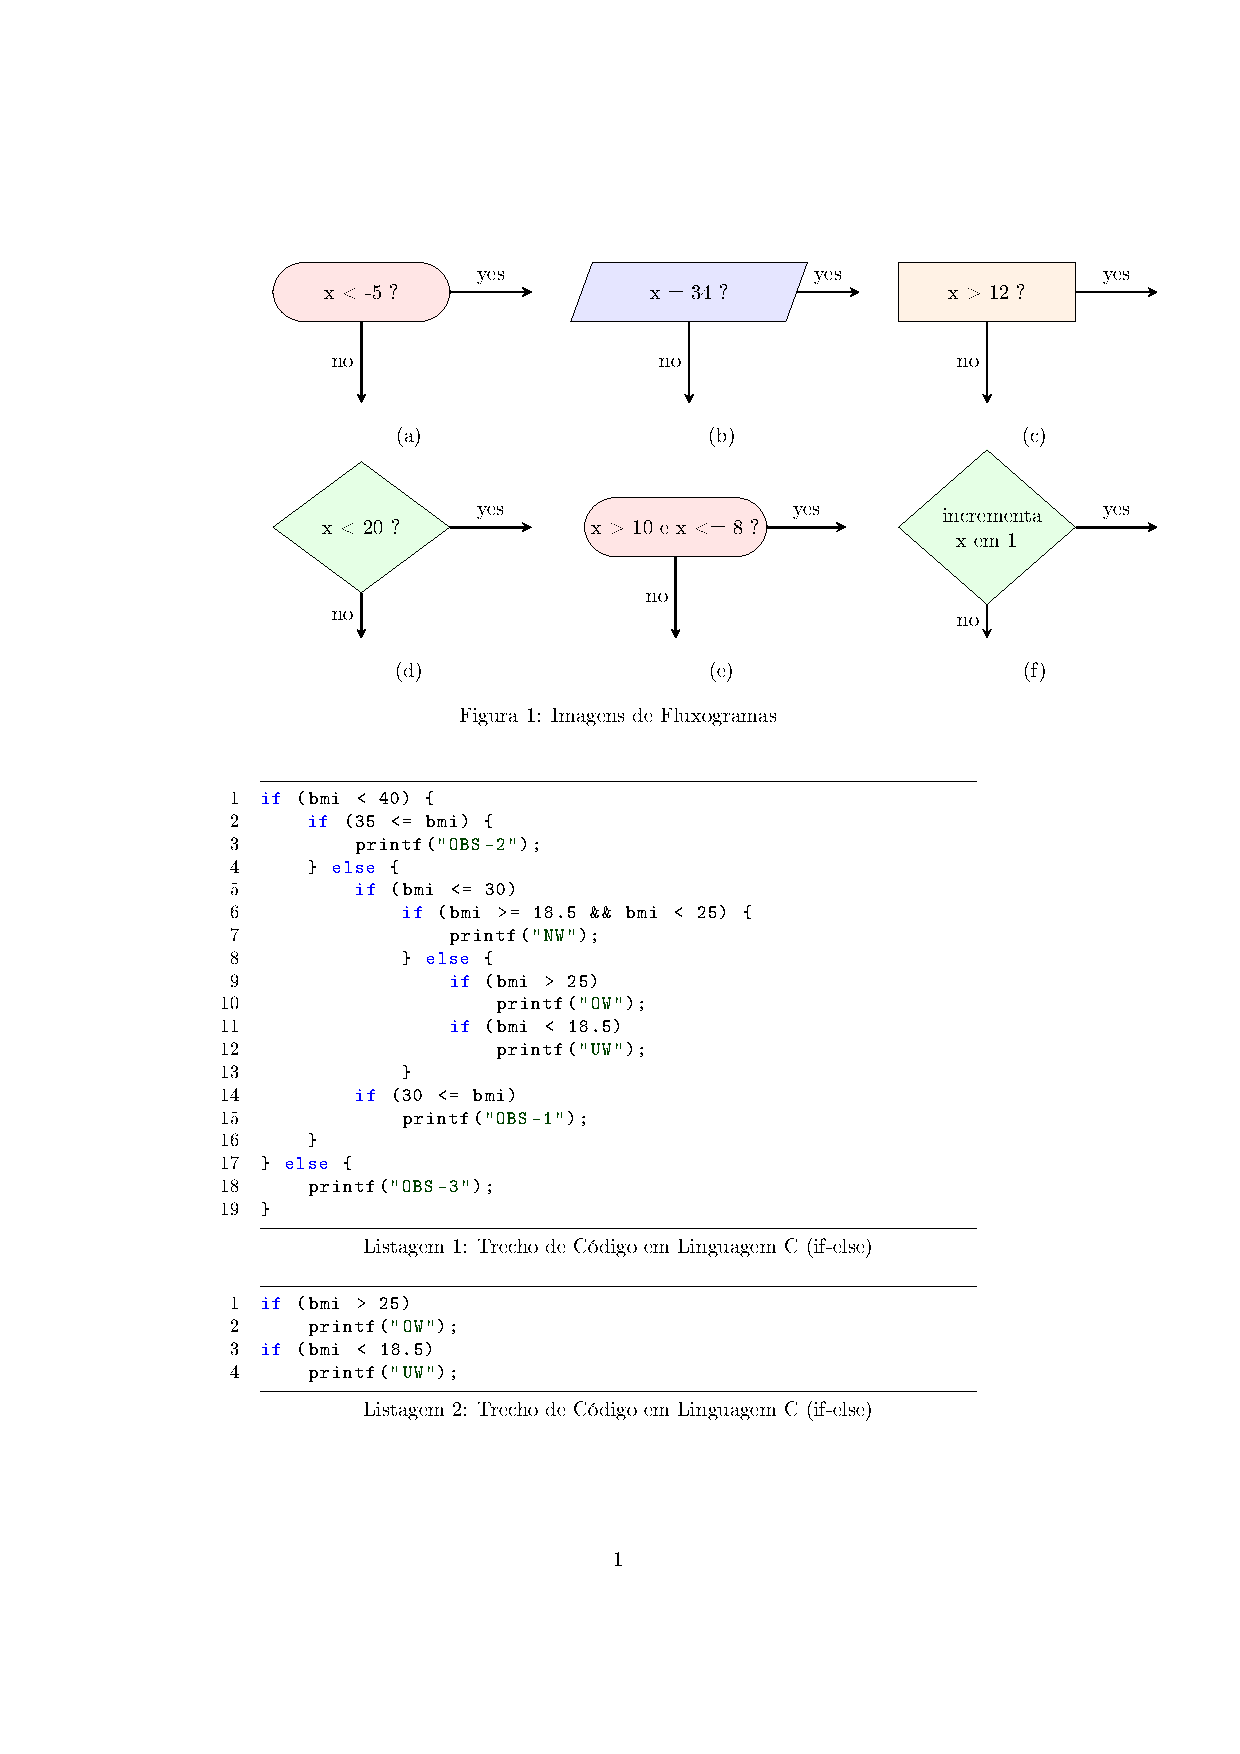
\includegraphics[page=1,width=1\textwidth]{images/annex/first-study-pre-list.pdf}

\newpage
\section{Programming Problem: Develop a Simple Virtual Temperature Monitor (P1)}
\label{annex:first-study-p1}
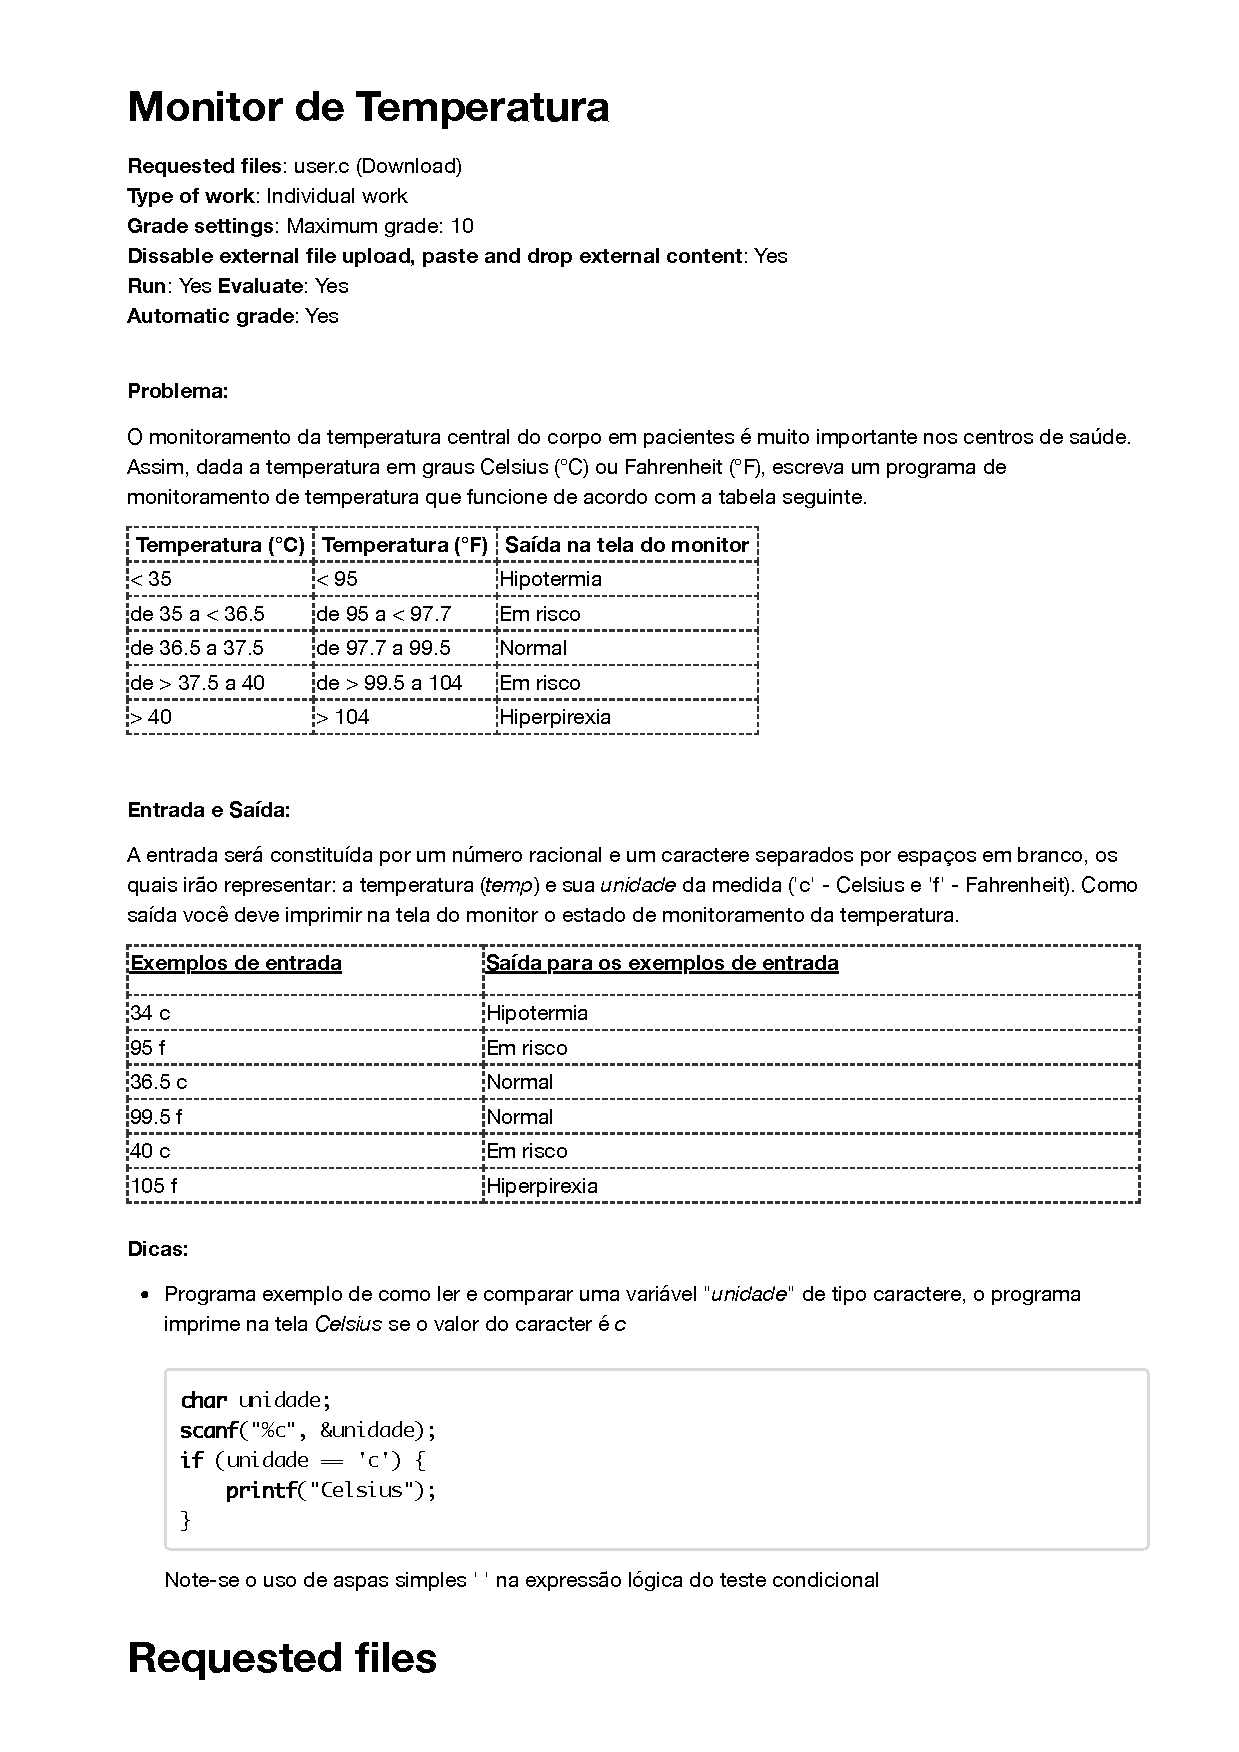
\includegraphics[page=1,width=1\textwidth]{images/annex/first-study-p1.pdf}

\newpage
\section{Formative Evaluation: Multiple Choice Knowledge Questionnaires of Cond. Structures (provinha1b)}
\label{annex:first-study-pos}
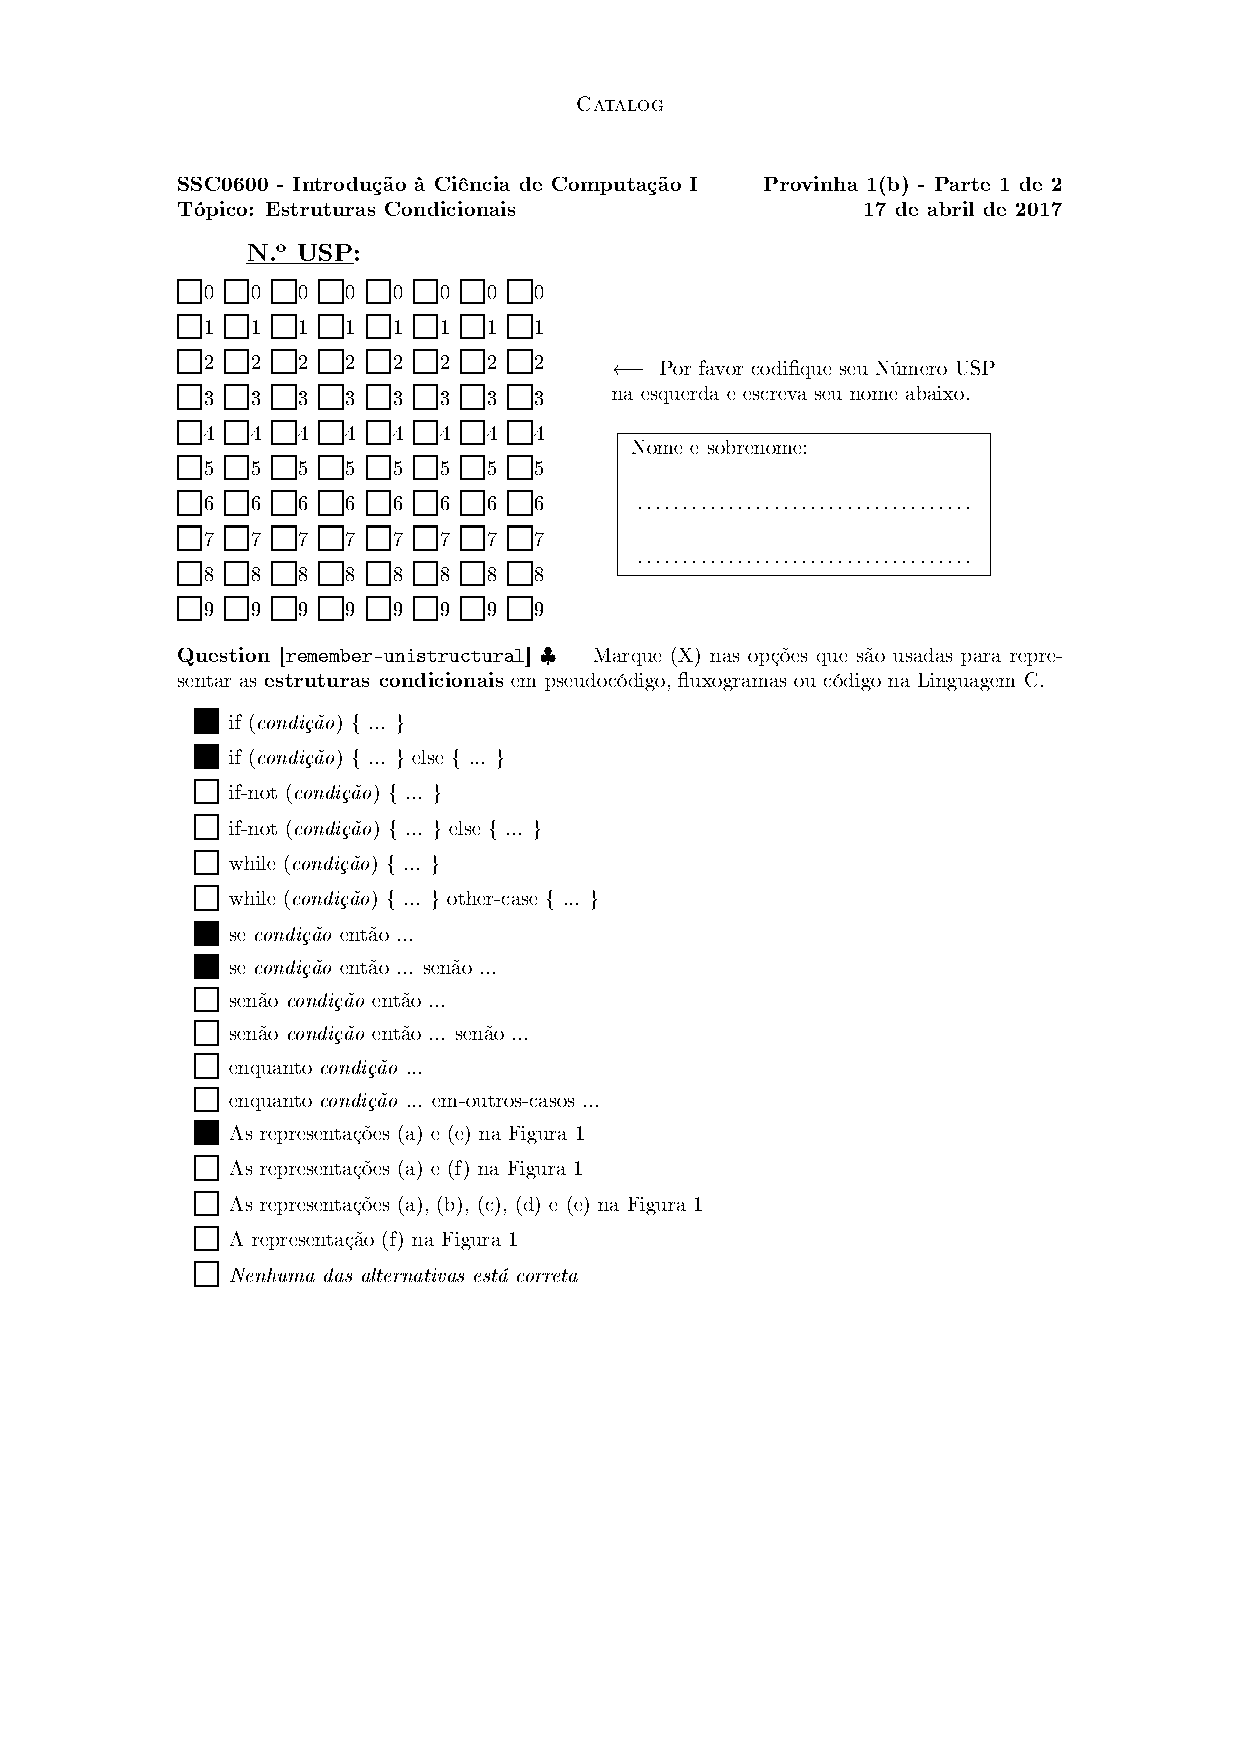
\includegraphics[page=1,width=1\textwidth]{images/annex/first-study-pos-1.pdf}
\newpage
\includegraphics[page=2,width=1\textwidth]{images/annex/first-study-pos-1.pdf}
\newpage
\includegraphics[page=3,width=1\textwidth]{images/annex/first-study-pos-1.pdf}
\newpage
\includegraphics[page=4,width=1\textwidth]{images/annex/first-study-pos-1.pdf}
\newpage
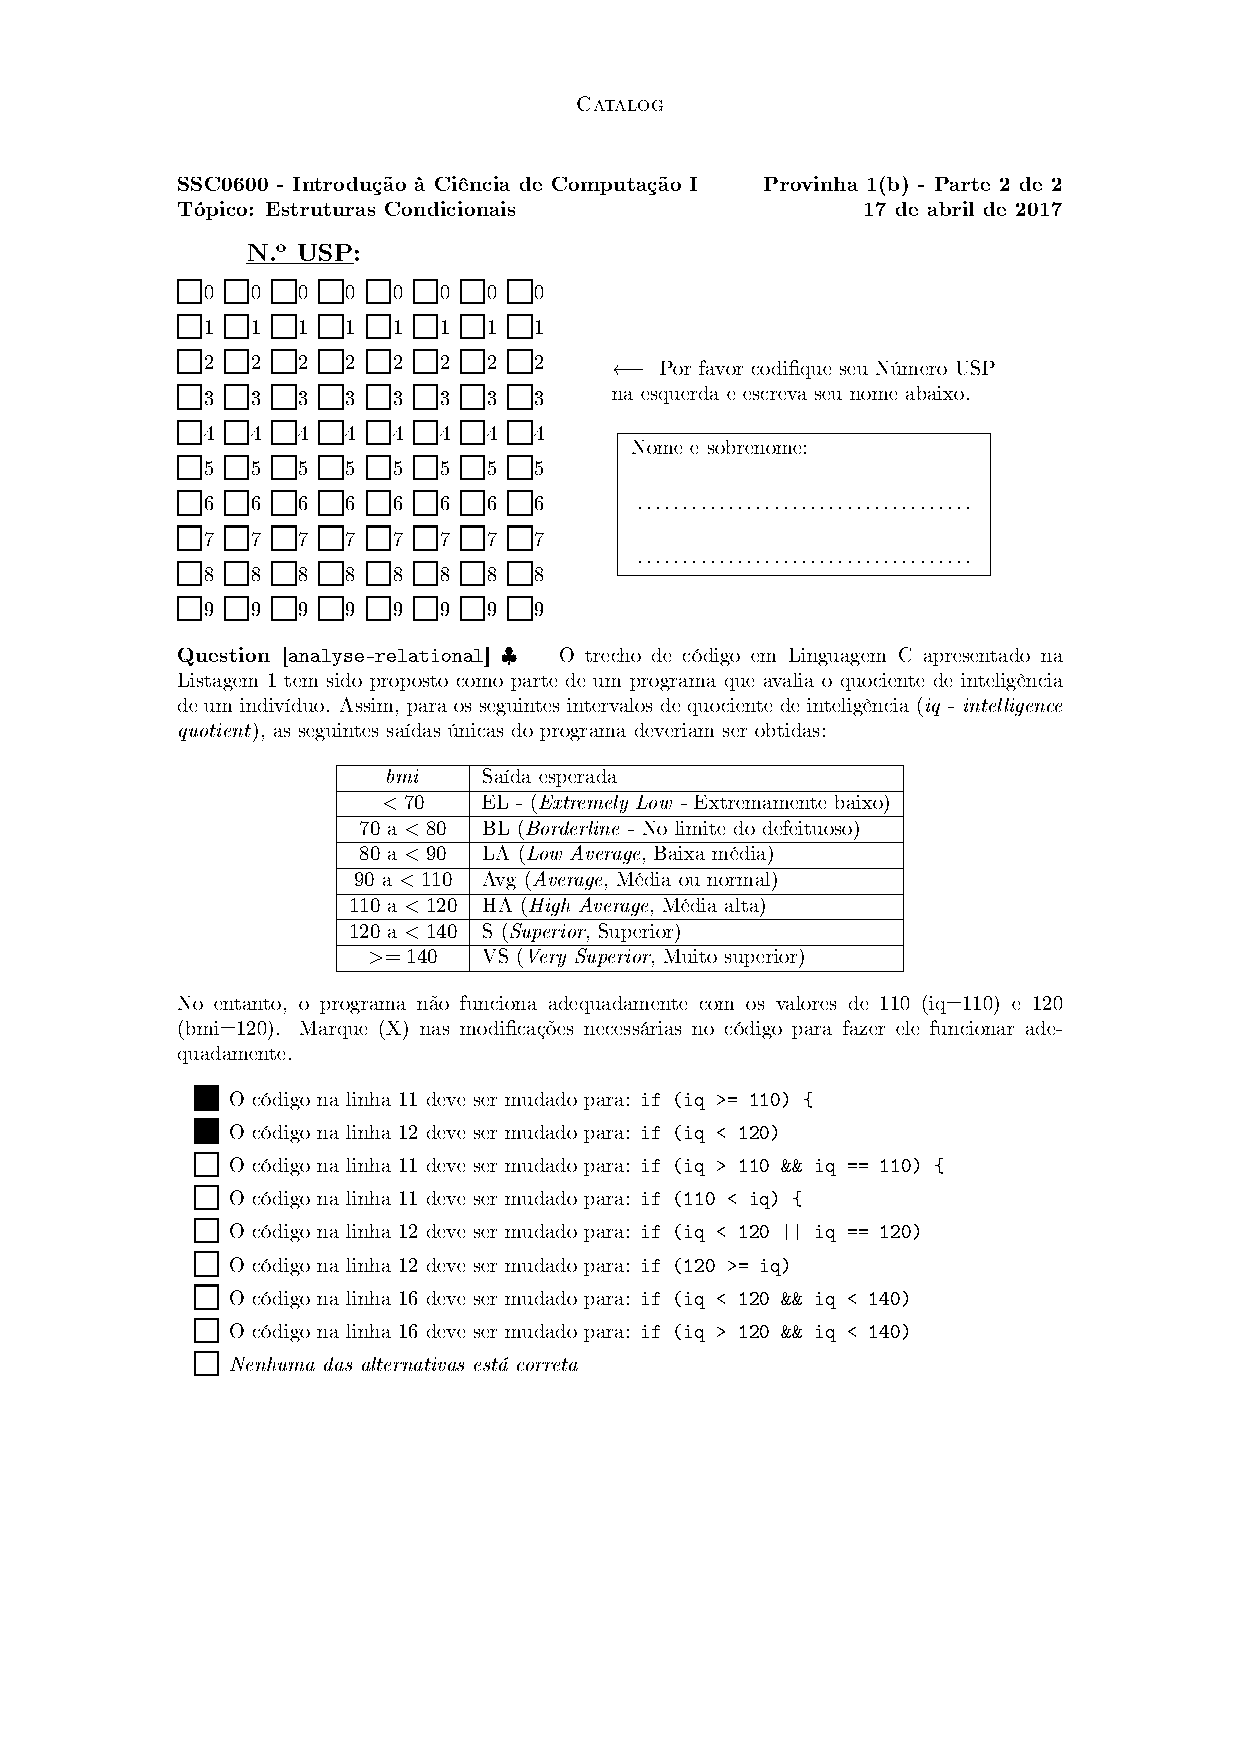
\includegraphics[page=1,width=1\textwidth]{images/annex/first-study-pos-2.pdf}
\newpage
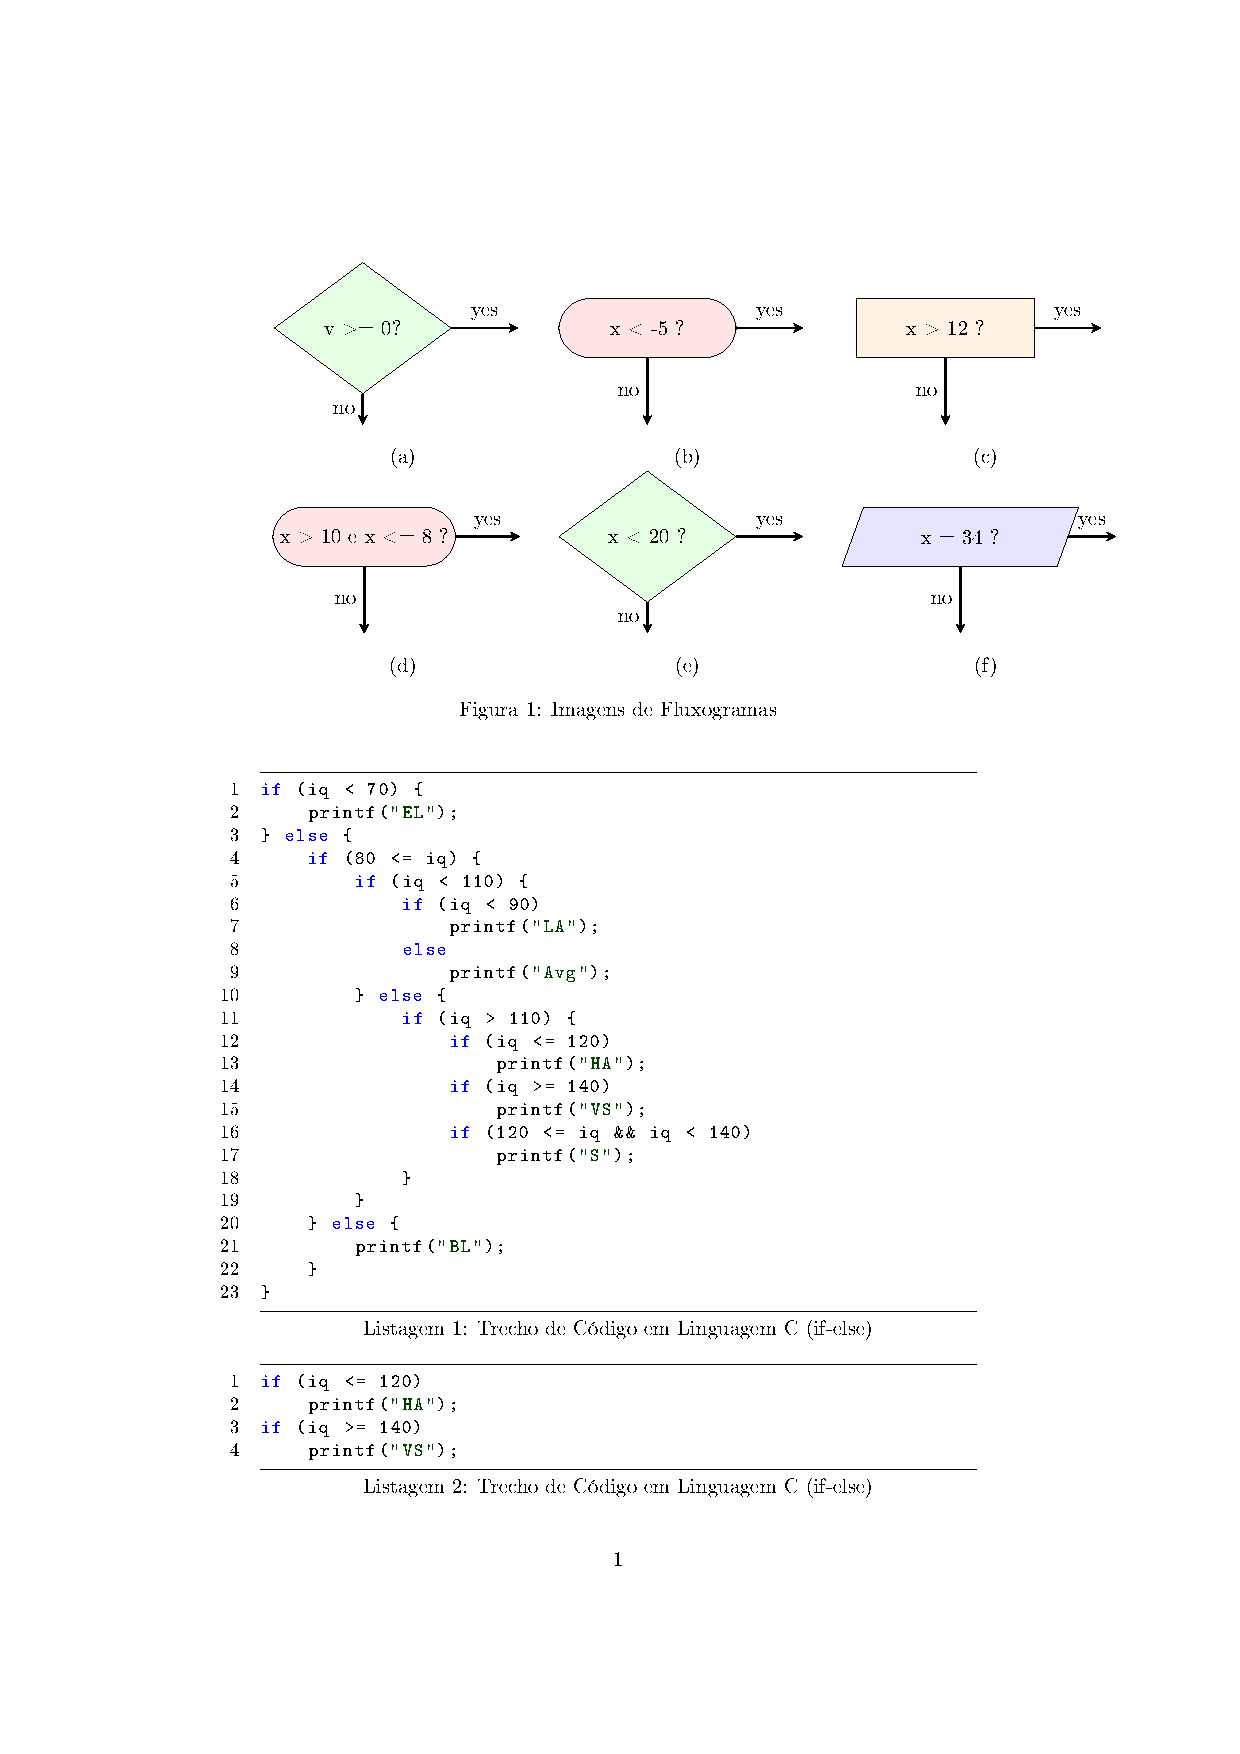
\includegraphics[page=1,width=1\textwidth]{images/annex/first-study-pos-list.pdf}

\newpage
\section{Programming Problem: Develop a Basal Metabolic Rate (PA)}
\label{annex:first-study-pA}
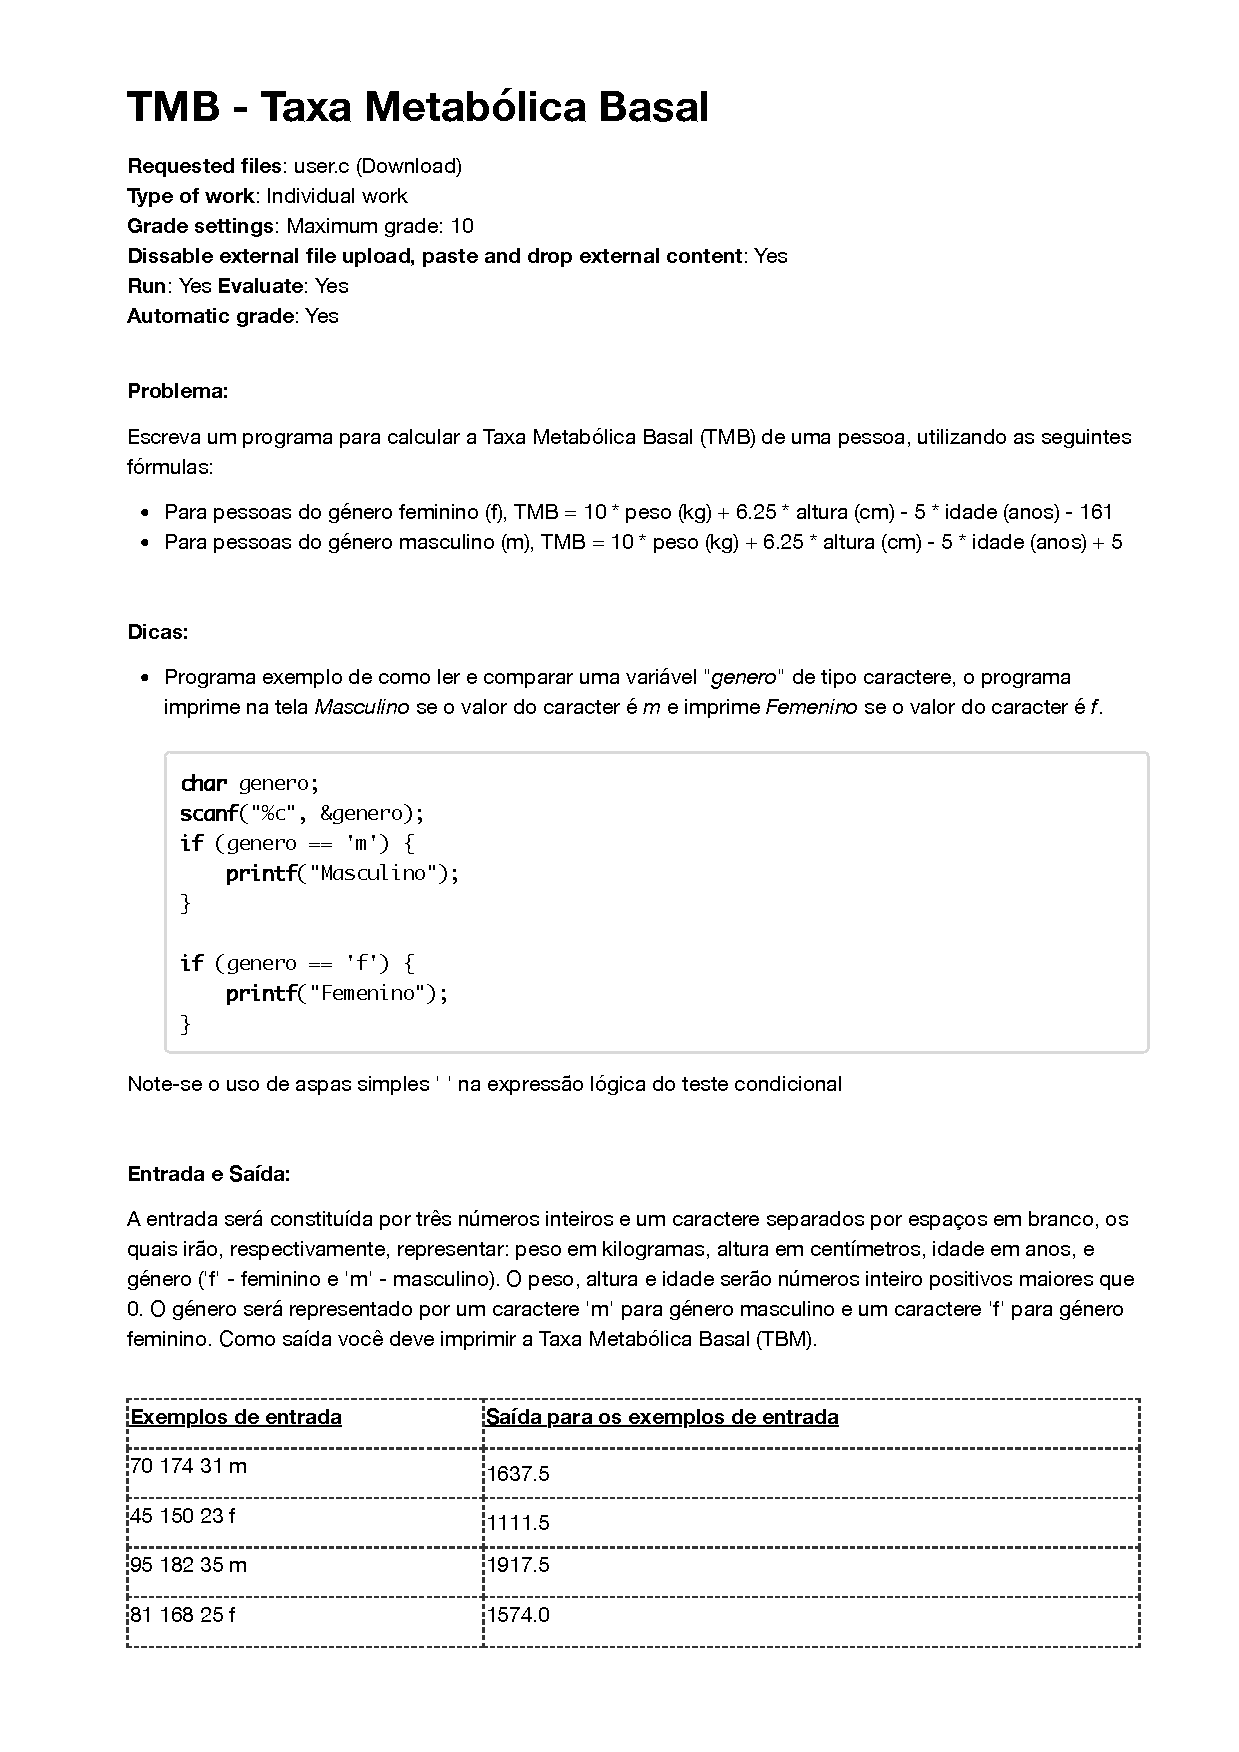
\includegraphics[page=1,width=1\textwidth]{images/annex/first-study-pA.pdf}

\newpage
\section{Programming Problem: Develop a Diet Calculator (PB)}
\label{annex:first-study-pB}
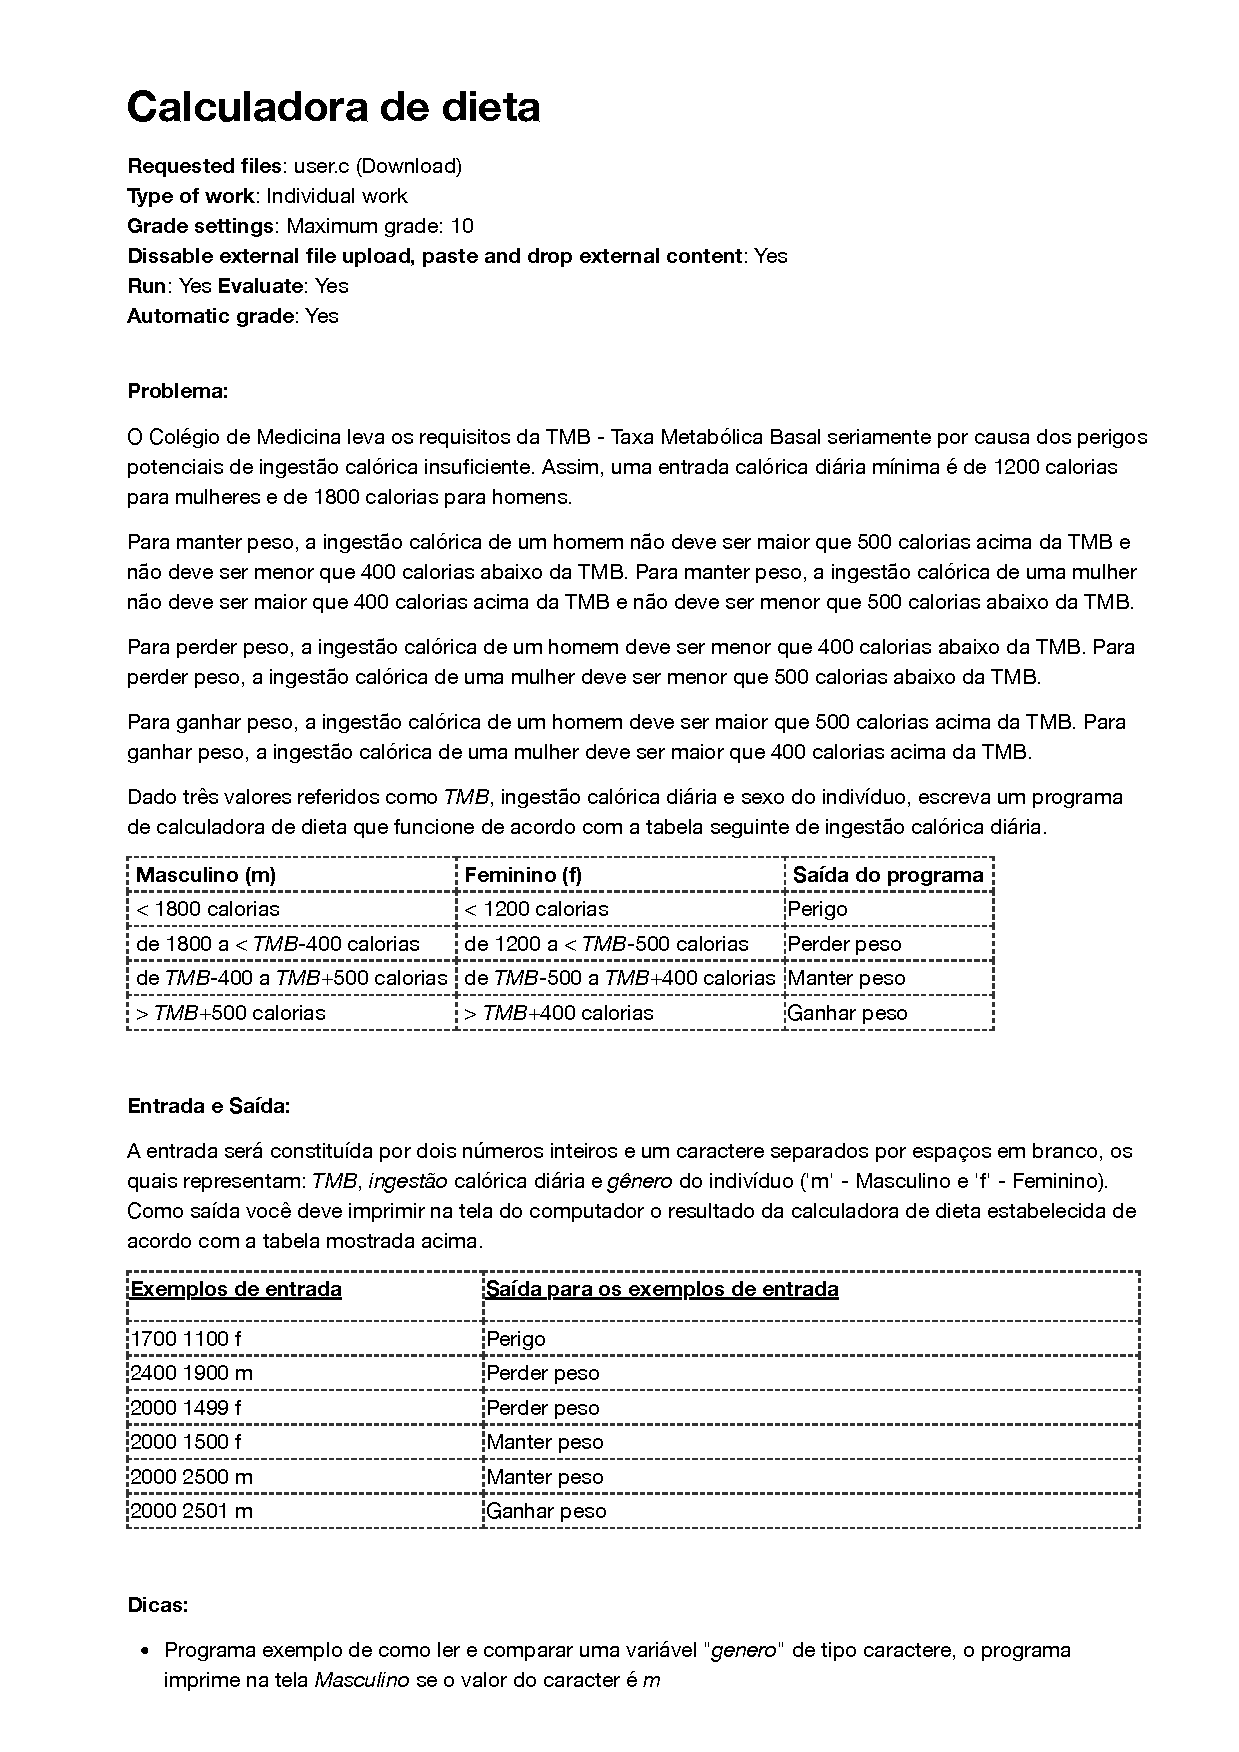
\includegraphics[page=1,width=1\textwidth]{images/annex/first-study-pB.pdf}

%%
\newpage
\section{Formative Evaluation: Multiple Choice Knowledge Questionnaires of Loop Structures (provinha2a)}
\label{annex:second-study-pre}
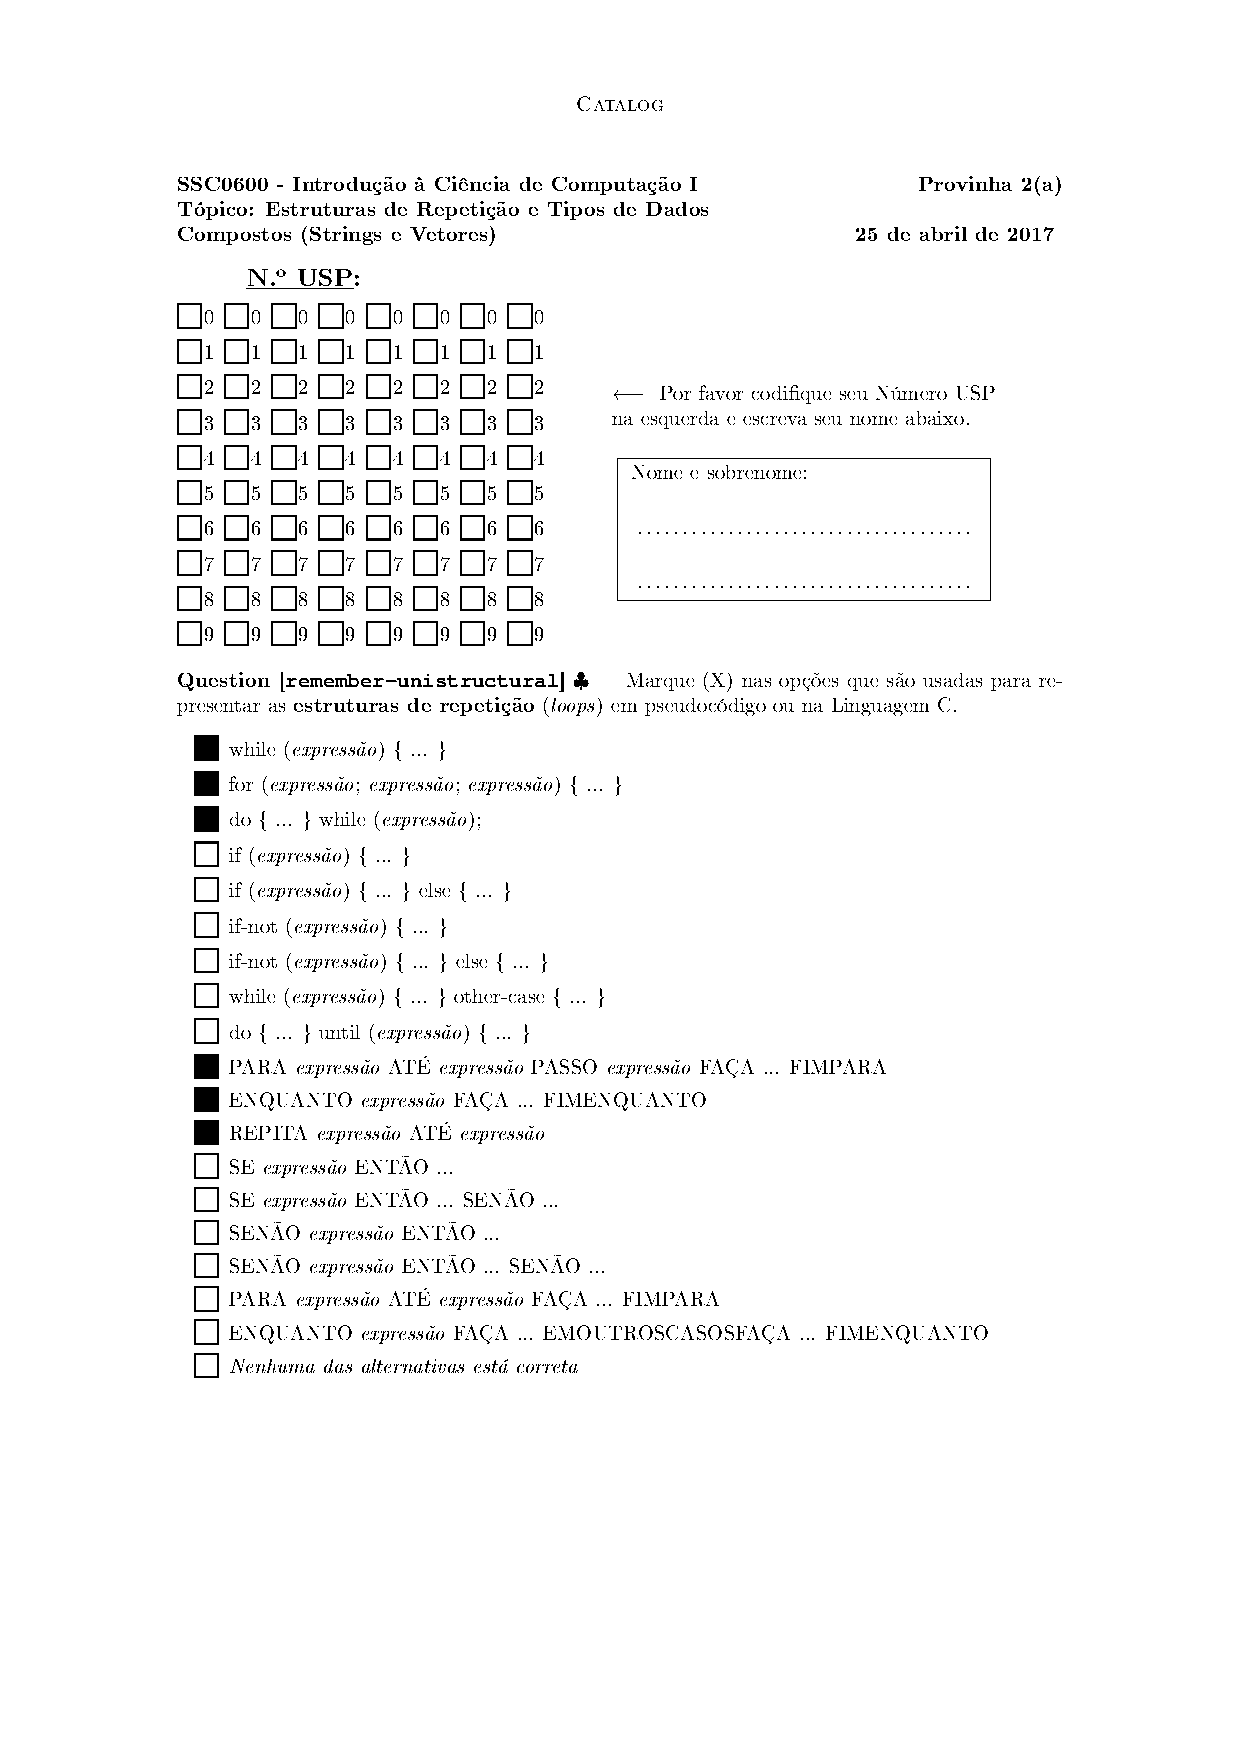
\includegraphics[page=1,width=1\textwidth]{images/annex/second-study-pre.pdf}
\newpage
\includegraphics[page=2,width=1\textwidth]{images/annex/second-study-pre.pdf}
\newpage
\includegraphics[page=3,width=1\textwidth]{images/annex/second-study-pre.pdf}
\newpage
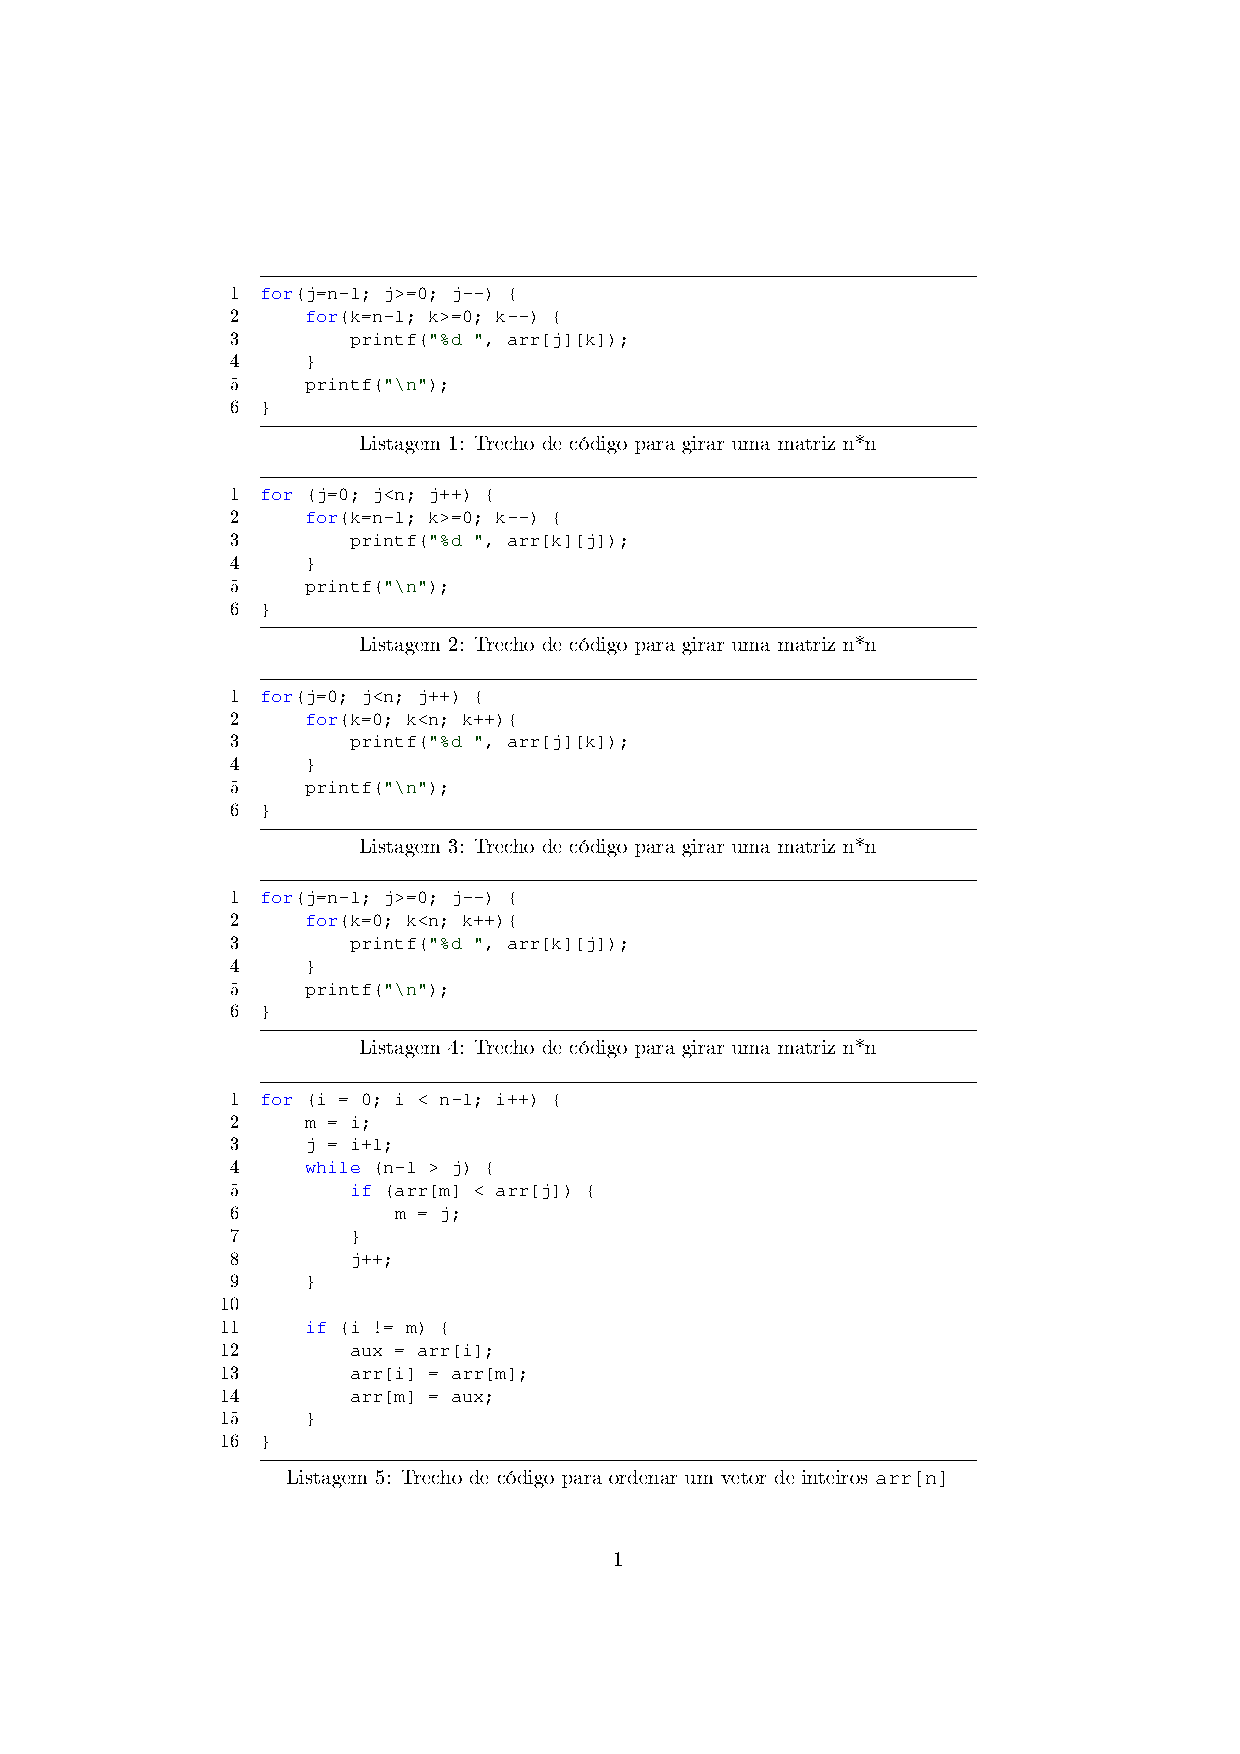
\includegraphics[page=1,width=1\textwidth]{images/annex/second-study-pre-list.pdf}
\newpage
\includegraphics[page=2,width=1\textwidth]{images/annex/second-study-pre-list.pdf}

\newpage
\section{Programming Problem: Calculate the Proper Divisors of a Number (P2)}
\label{annex:second-study-p2}
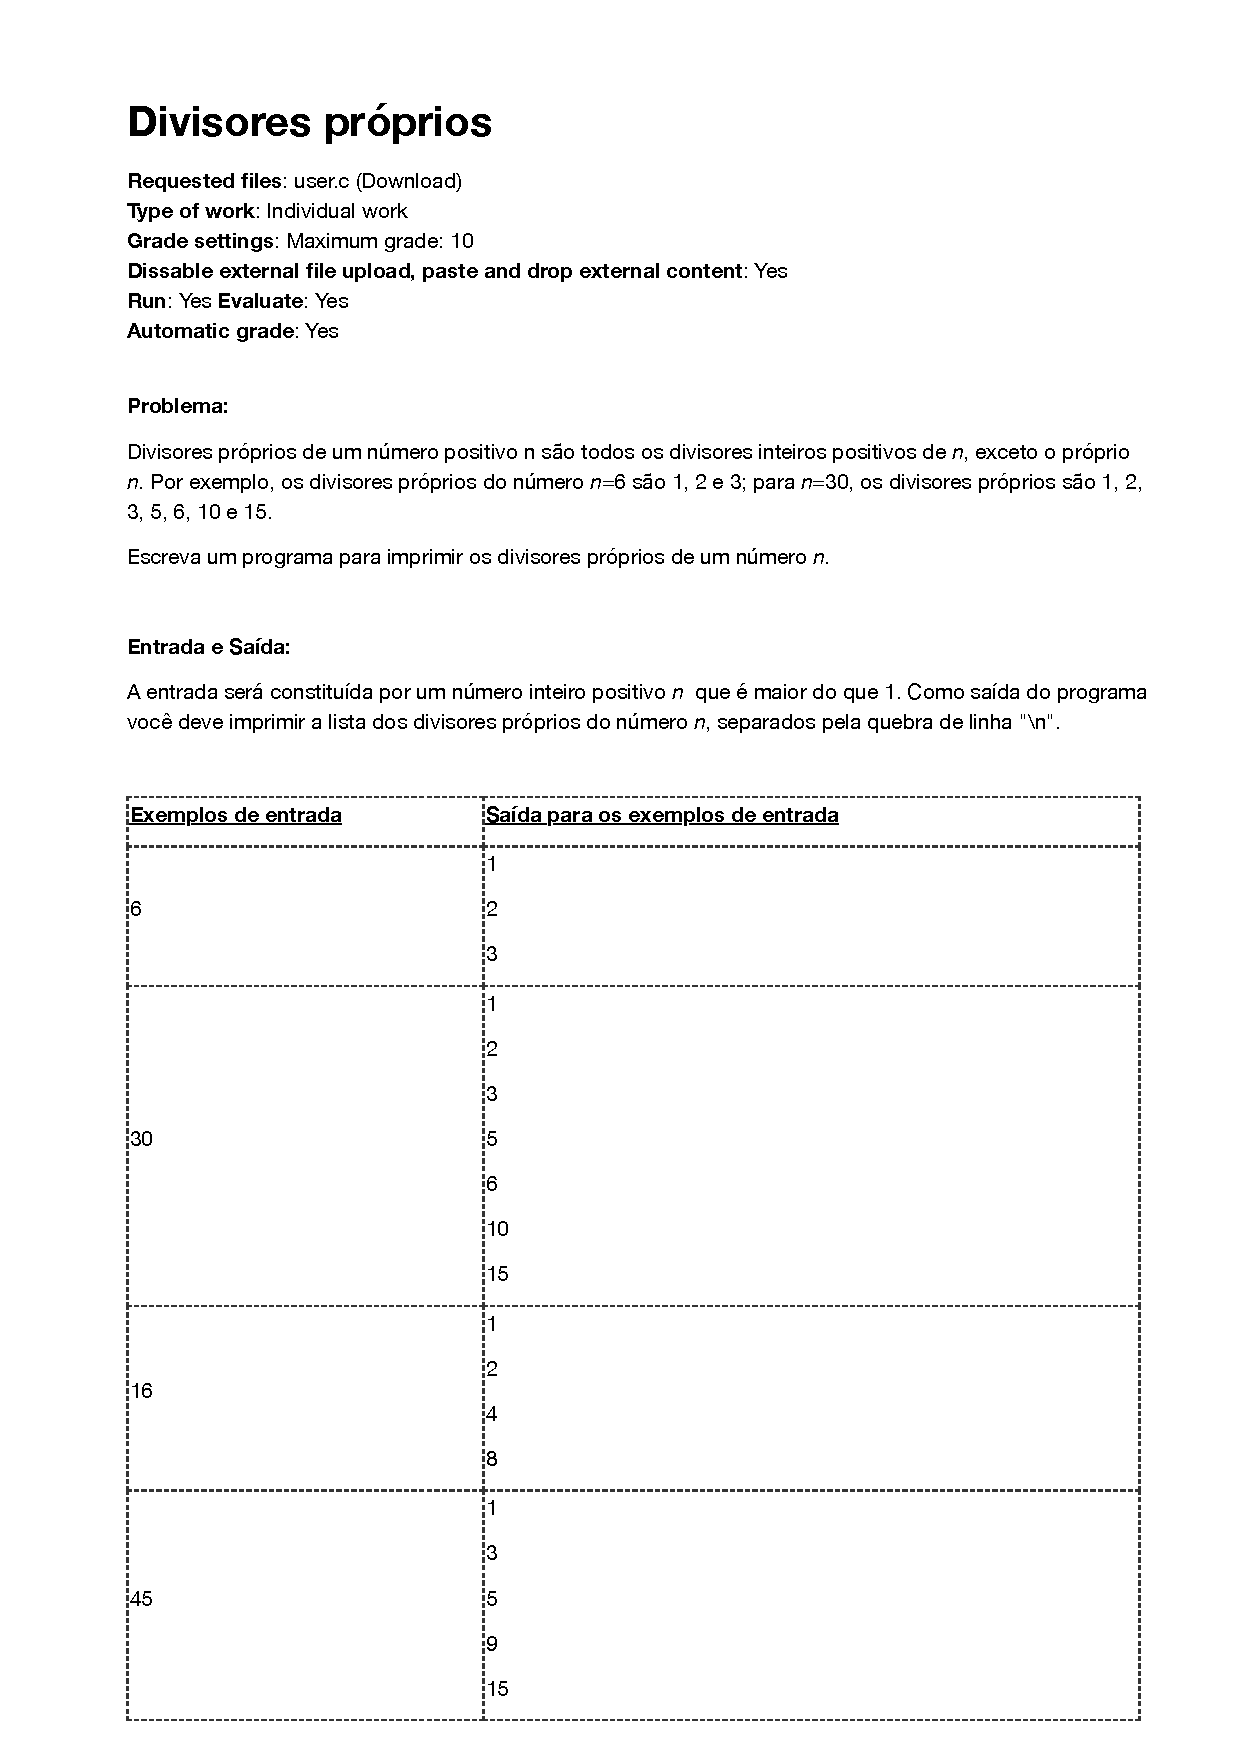
\includegraphics[page=1,width=1\textwidth]{images/annex/second-study-p2.pdf}

\newpage
\section{Programming Problem: Calculate the Maximum Length of a Hailstone Sequence (P3)}
\label{annex:second-study-p3}
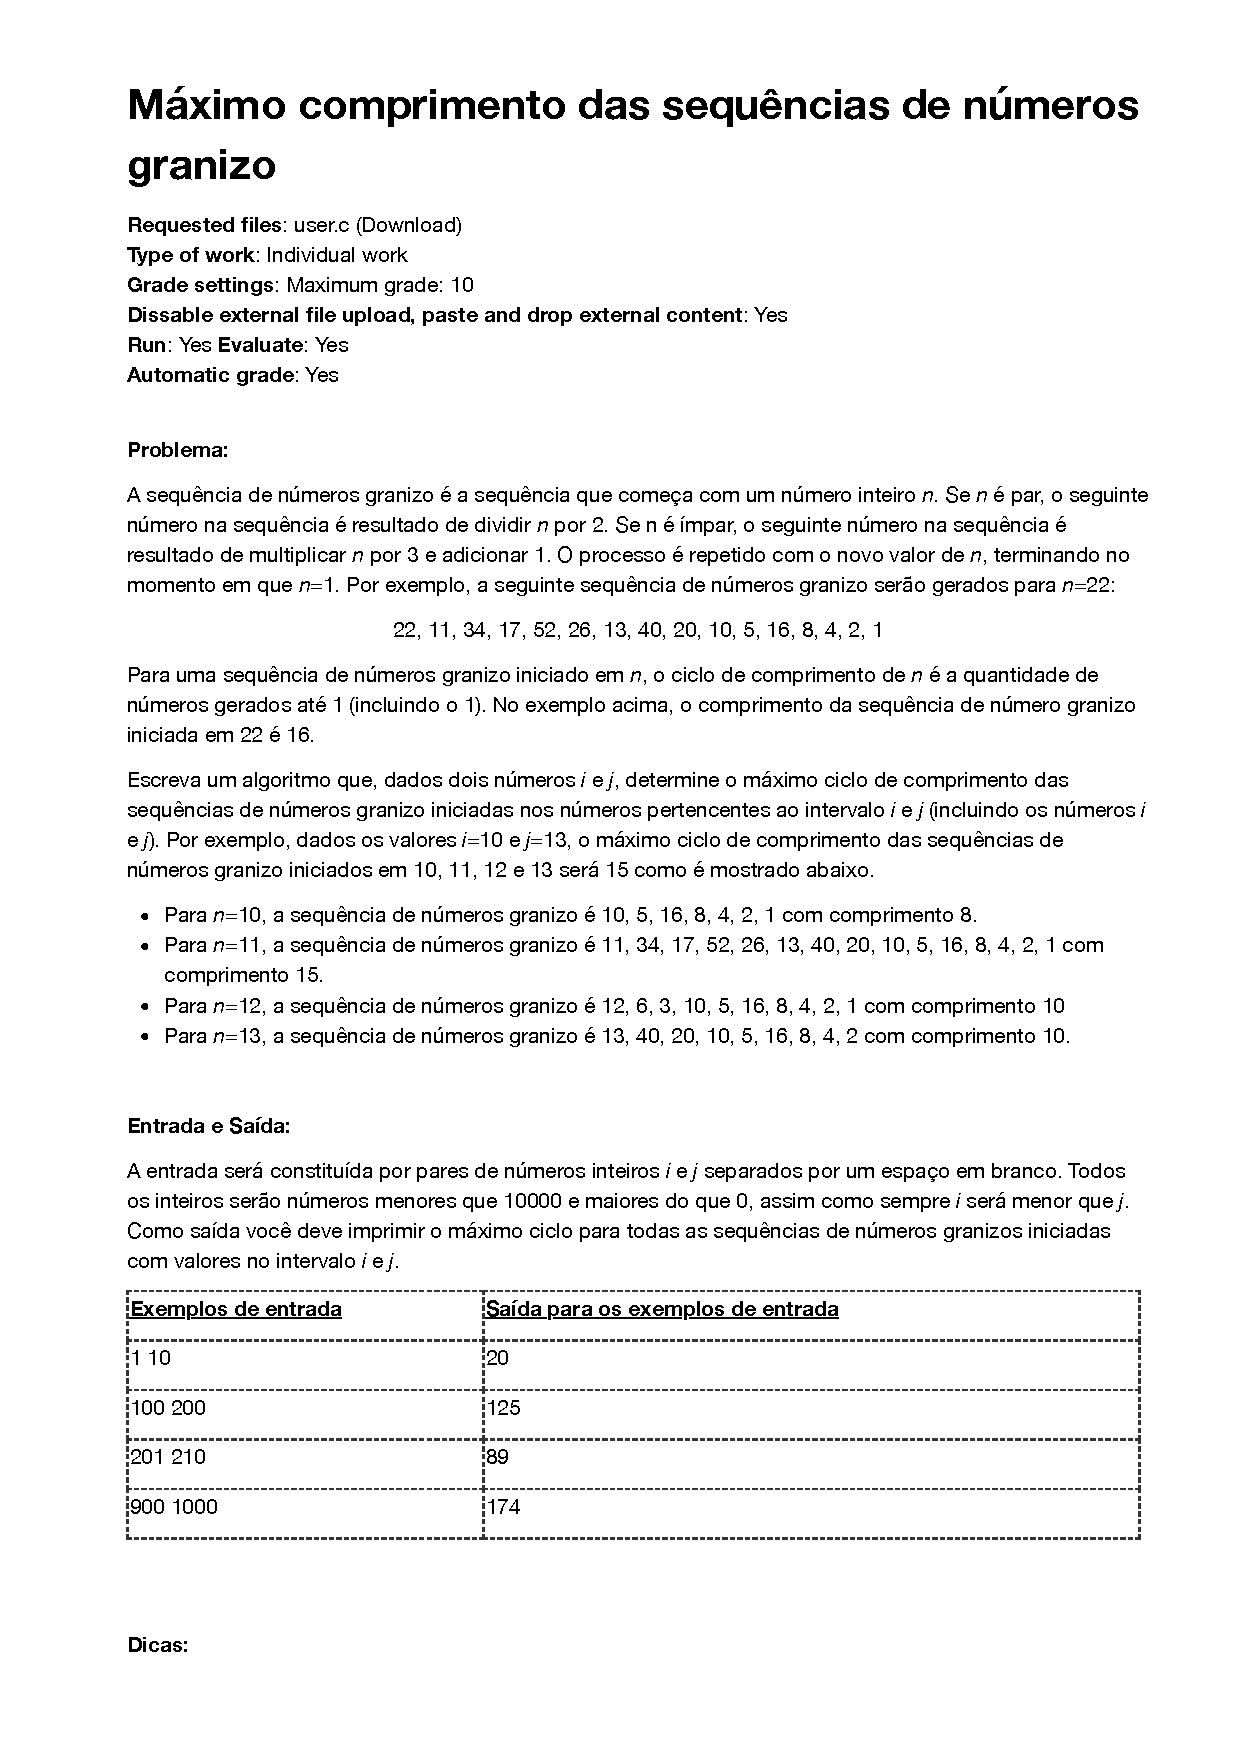
\includegraphics[page=1,width=1\textwidth]{images/annex/second-study-p3.pdf}

%%
\newpage
\section{Formative Evaluation: Multiple Choice Knowledge Questionnaires of Loop Structures (provinha2b)}
\label{annex:second-study-pos}
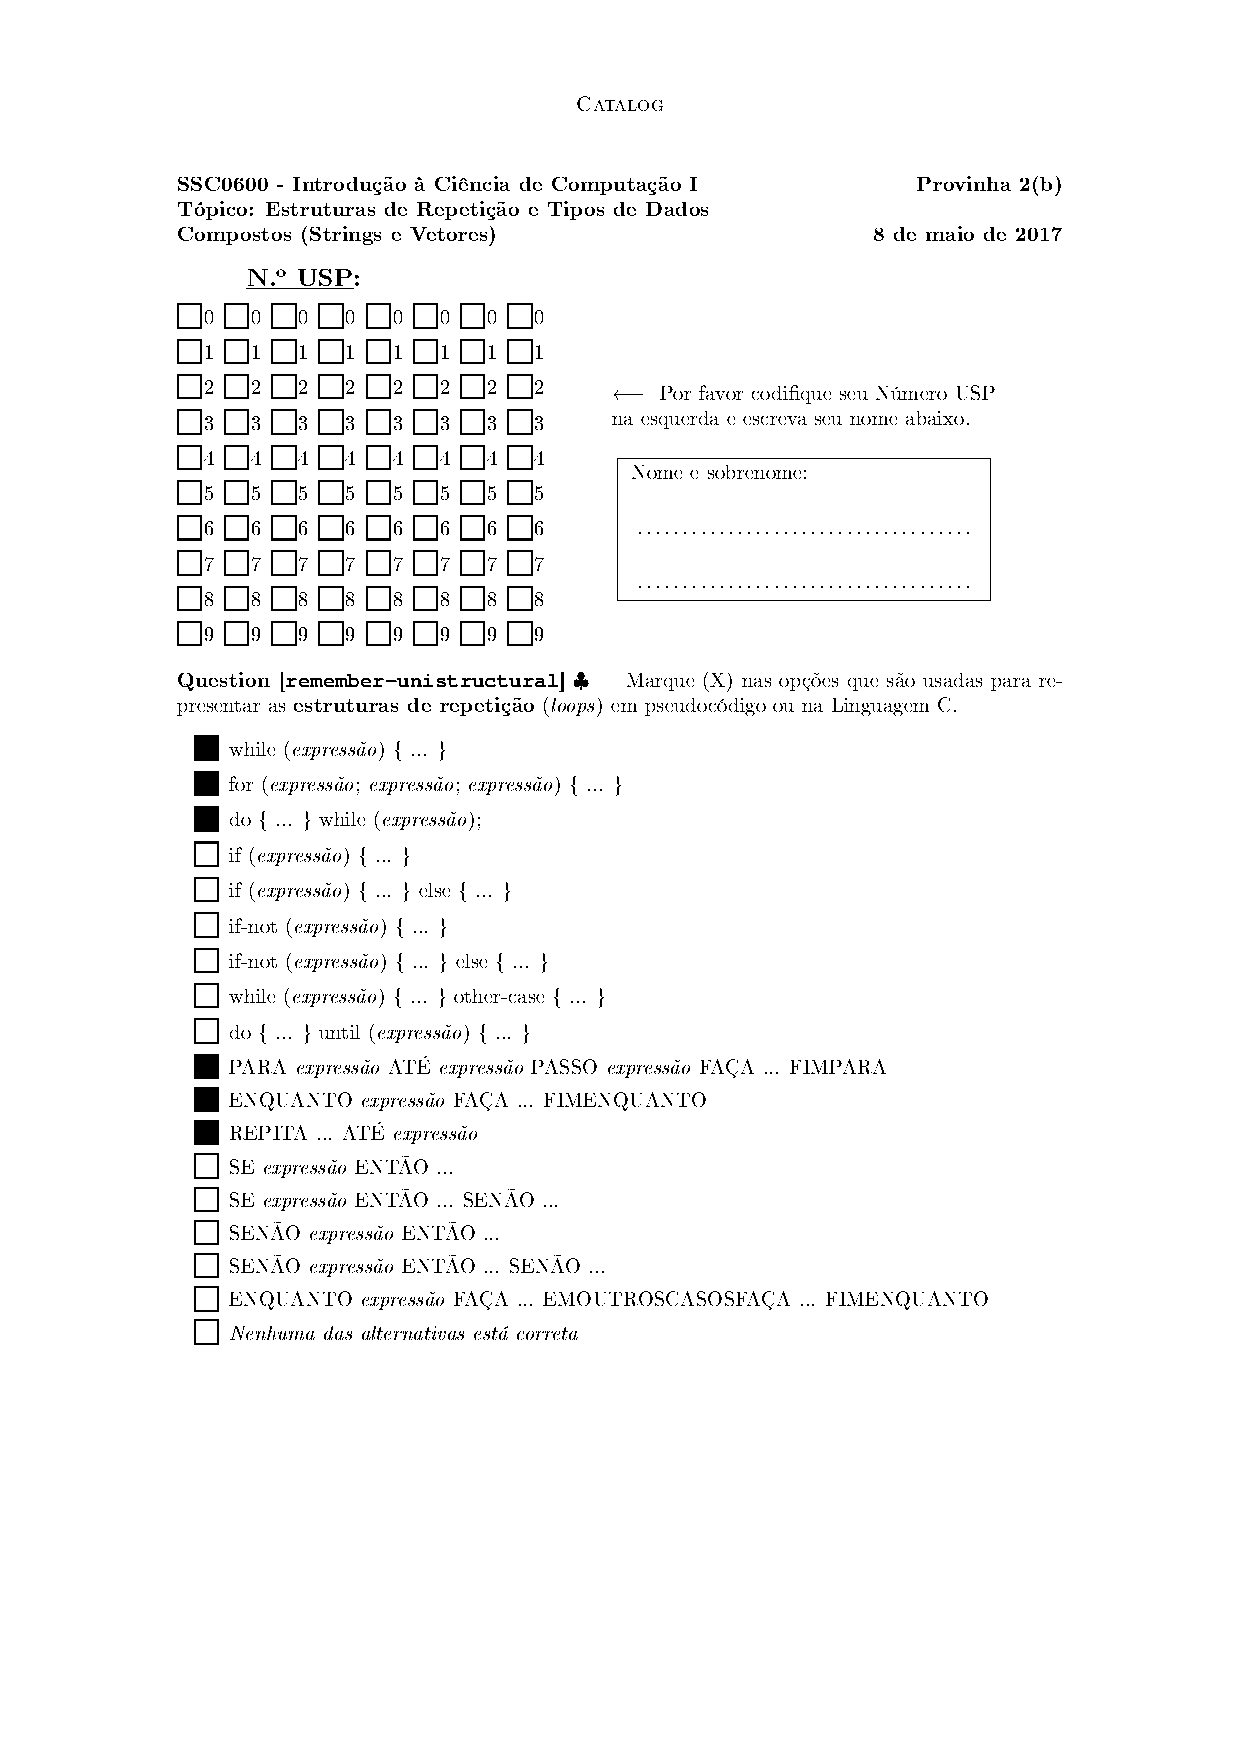
\includegraphics[page=1,width=1\textwidth]{images/annex/second-study-pos.pdf}
\newpage
\includegraphics[page=2,width=1\textwidth]{images/annex/second-study-pos.pdf}
\newpage
\includegraphics[page=3,width=1\textwidth]{images/annex/second-study-pos.pdf}
\newpage
\includegraphics[page=4,width=1\textwidth]{images/annex/second-study-pos.pdf}
\newpage
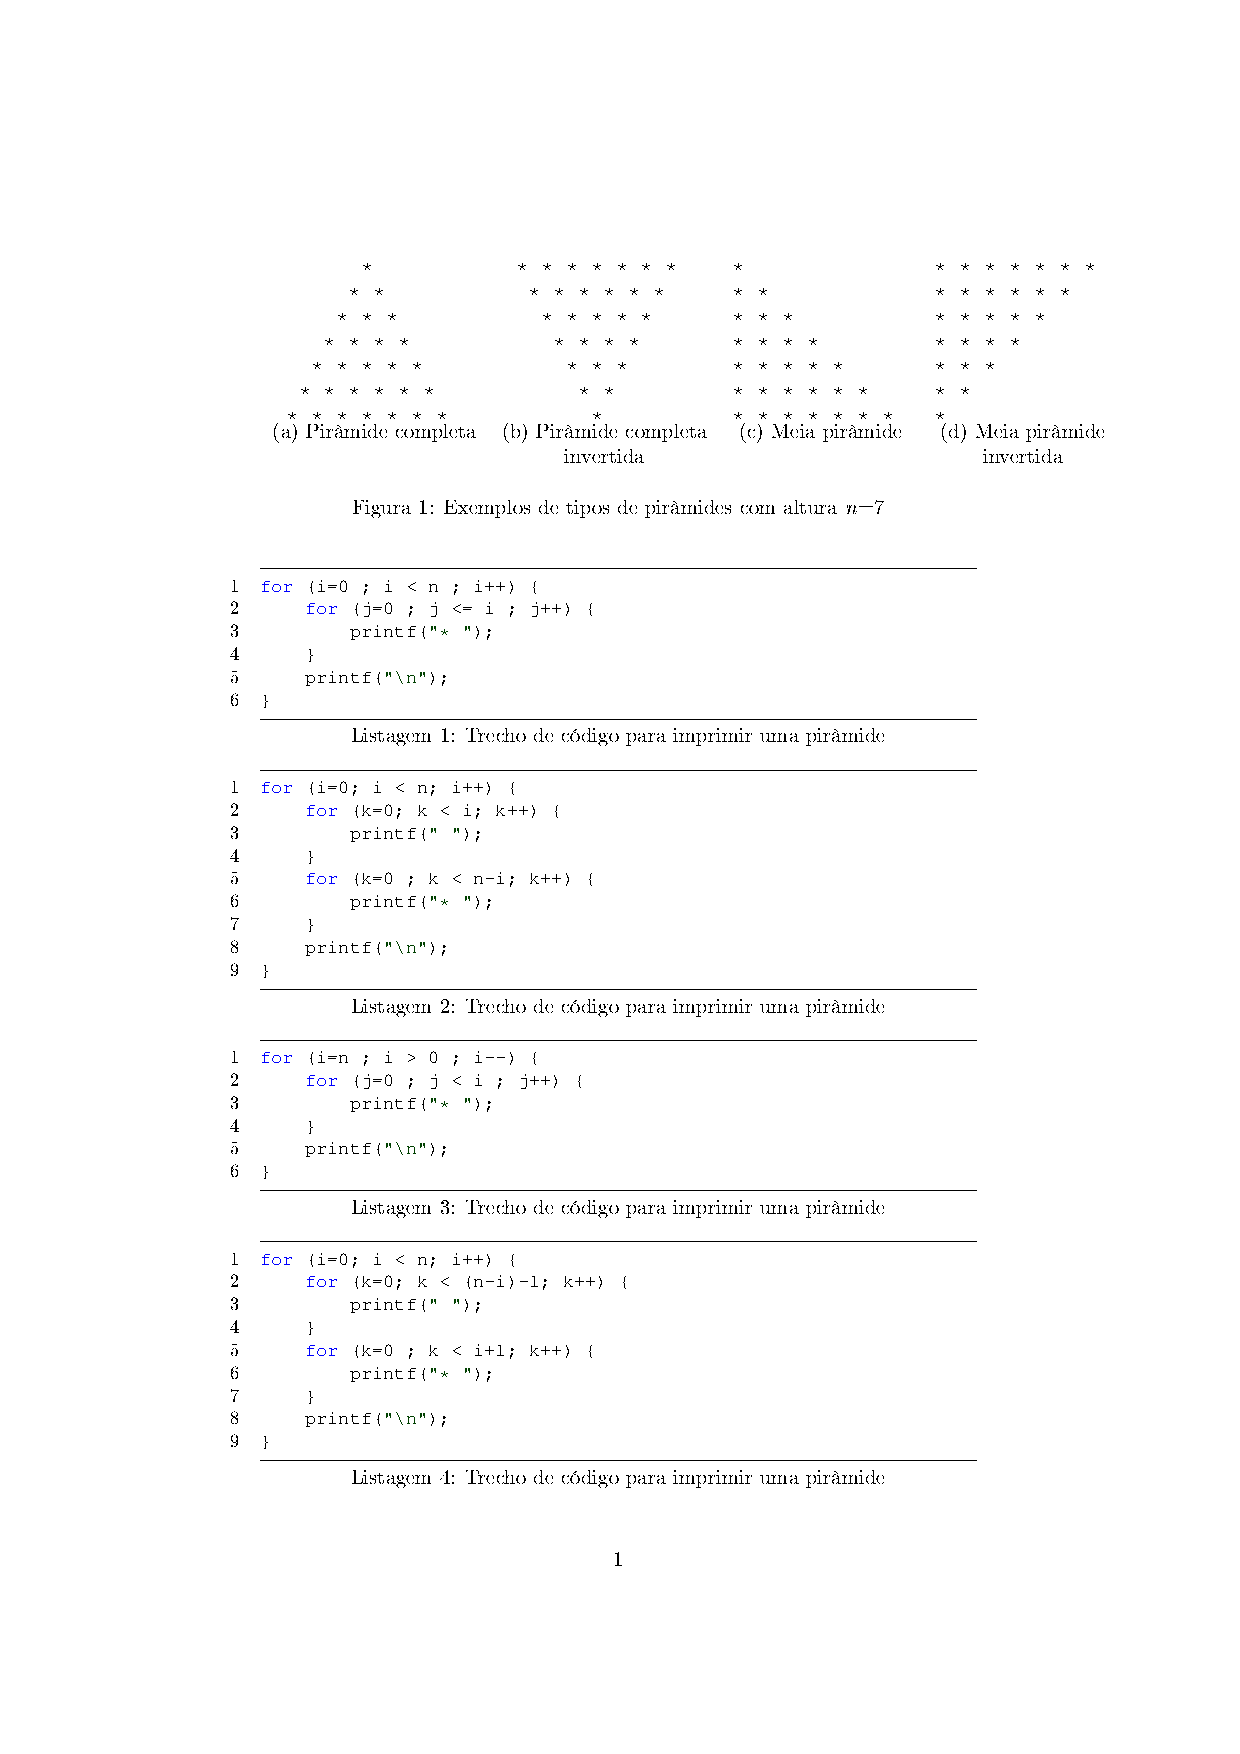
\includegraphics[page=1,width=1\textwidth]{images/annex/second-study-pos-list.pdf}
\newpage
\includegraphics[page=2,width=1\textwidth]{images/annex/second-study-pos-list.pdf}
\newpage
\includegraphics[page=3,width=1\textwidth]{images/annex/second-study-pos-list.pdf}

\newpage
\section{Programming Problem: Calculate a Geometric Sequence (PC)}
\label{annex:second-study-pC}
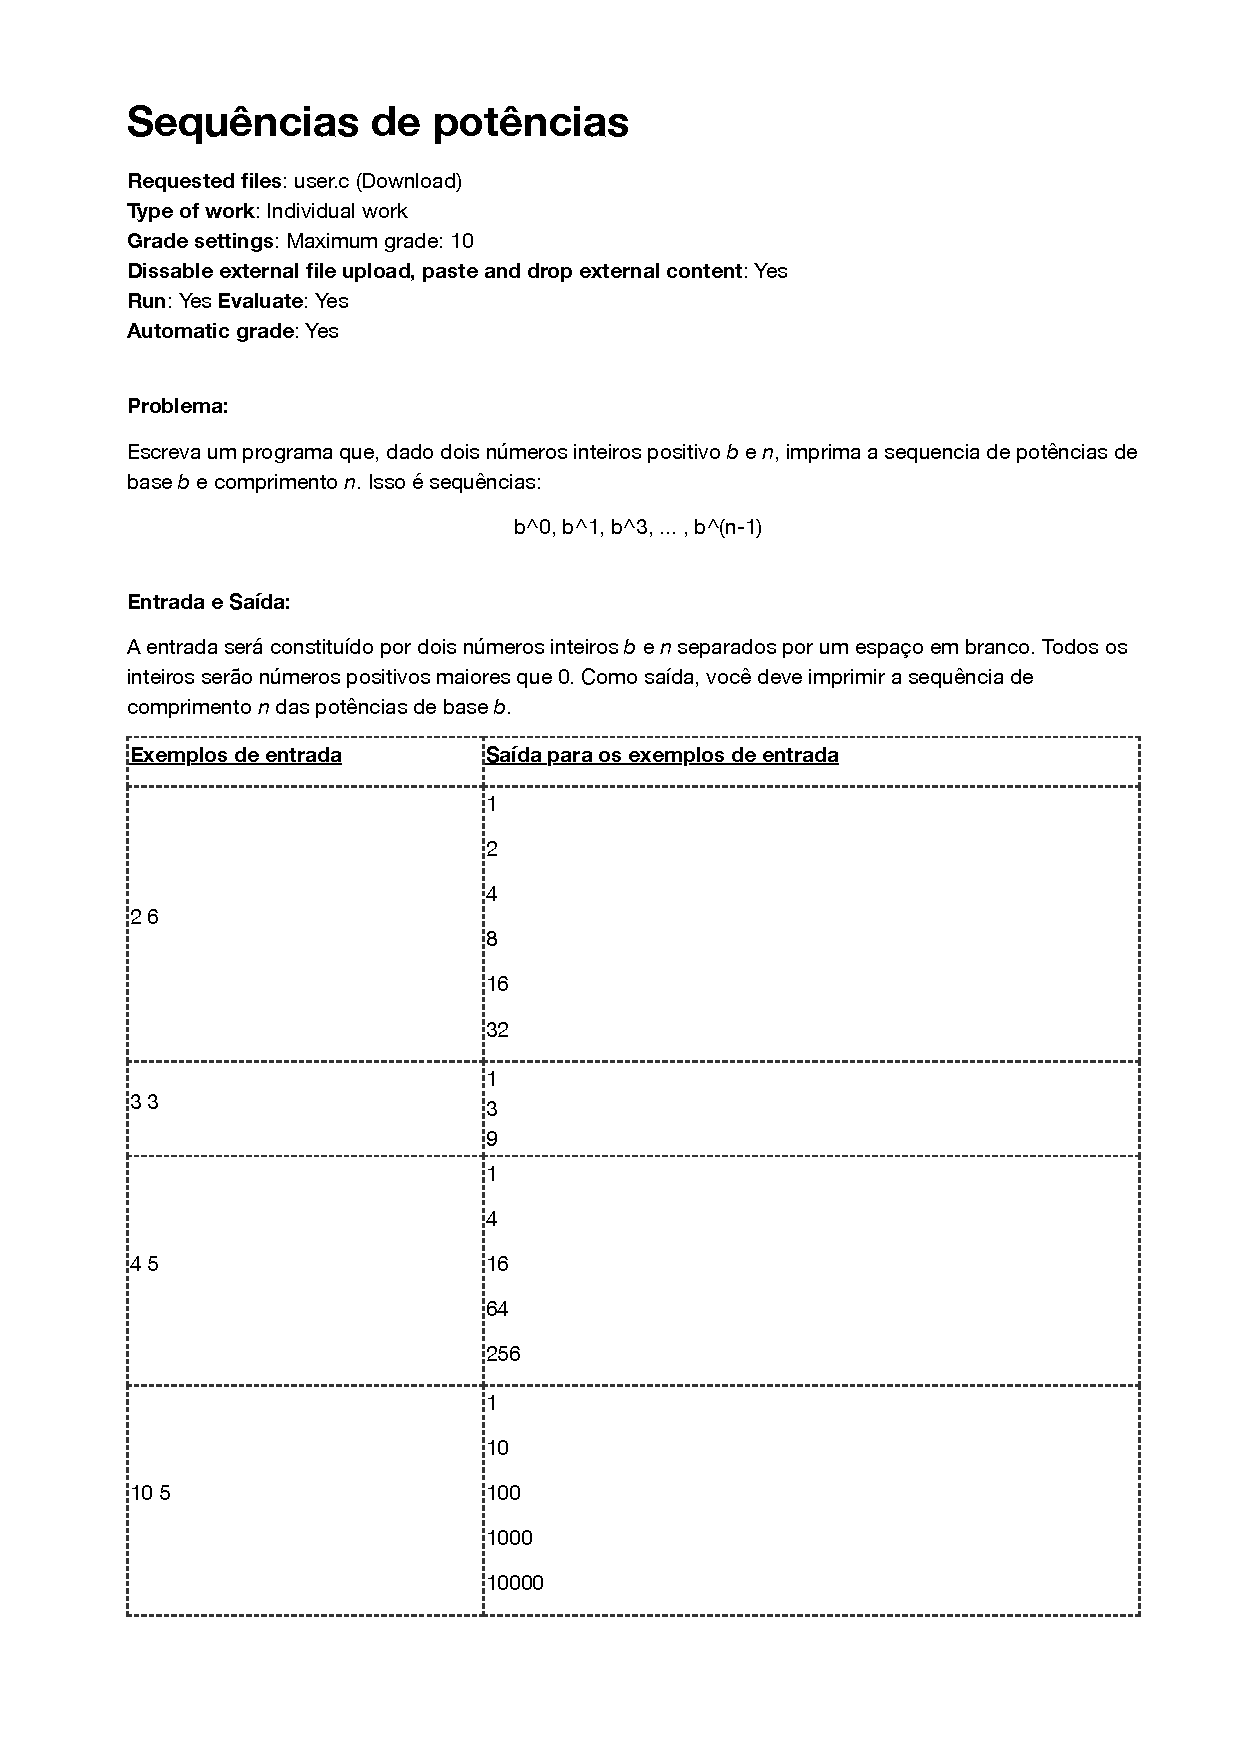
\includegraphics[page=1,width=1\textwidth]{images/annex/second-study-pC.pdf}

\newpage
\section{Programming Problem: Calculate Global Minimum Coin Changes (PD)}
\label{annex:second-study-pD}
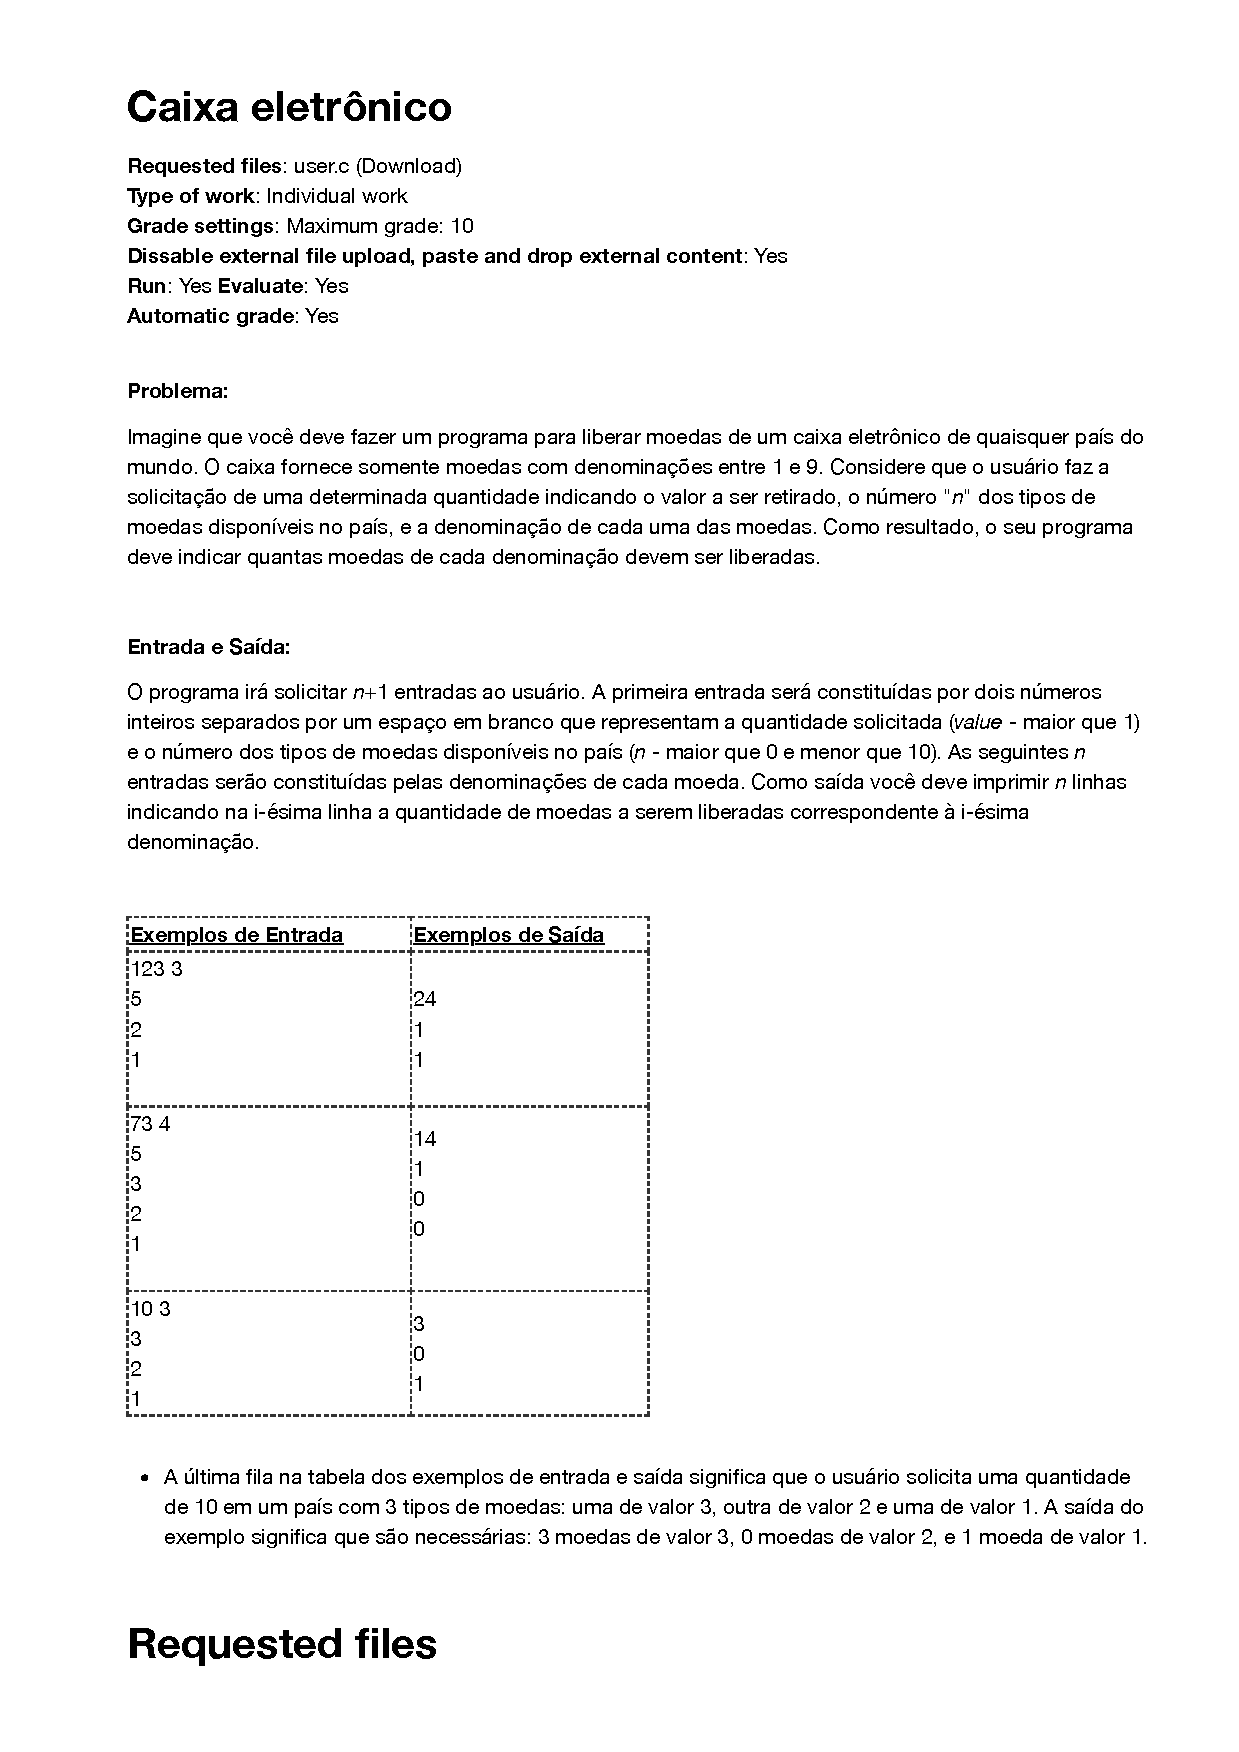
\includegraphics[page=1,width=1\textwidth]{images/annex/second-study-pD.pdf}

\newpage
\section{Programming Problem: Count Number of Semi-primes for RSA (PE)}
\label{annex:second-study-pE}
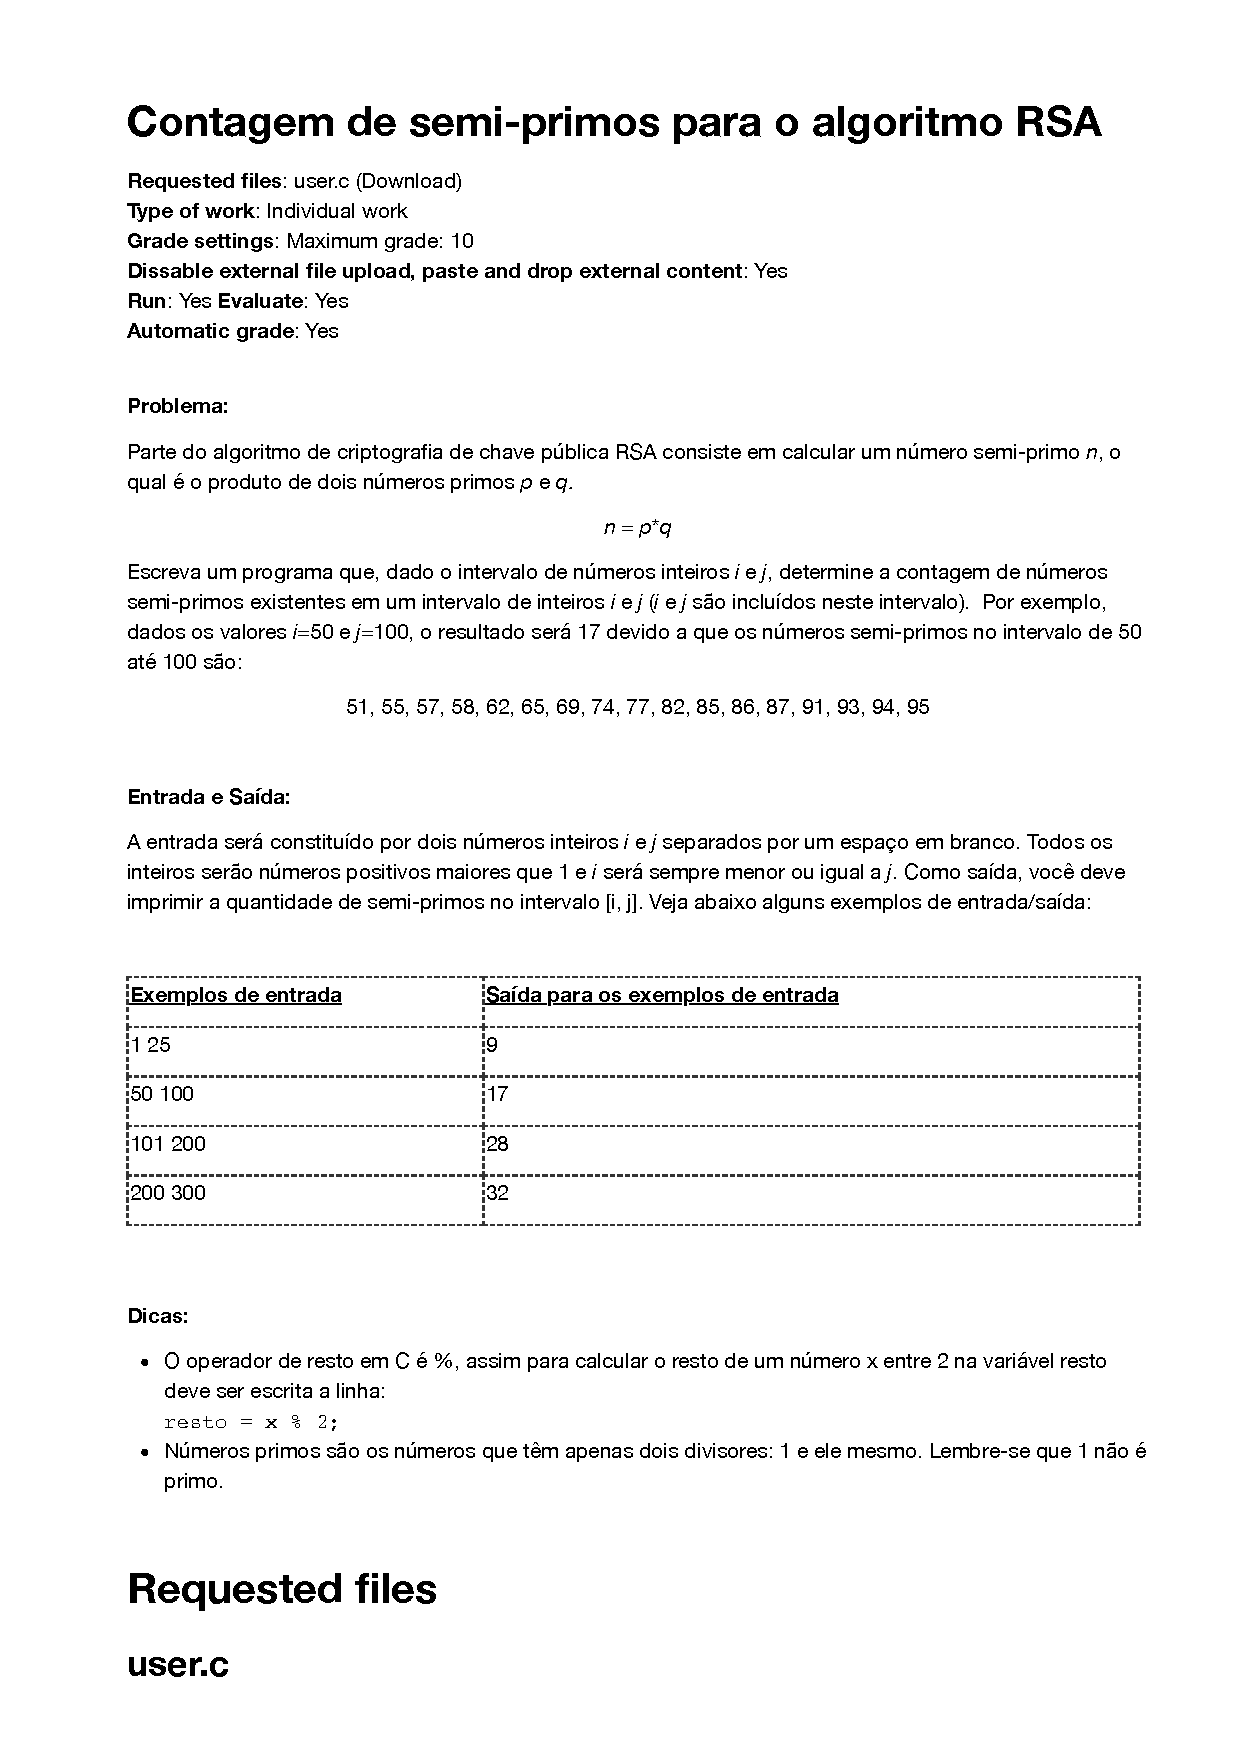
\includegraphics[page=1,width=1\textwidth]{images/annex/second-study-pE.pdf}

%%
\newpage
\section{Formative Evaluation: Multiple Choice Knowledge Questionnaires of Recursion (provinha3a)}
\label{annex:third-study-pre}
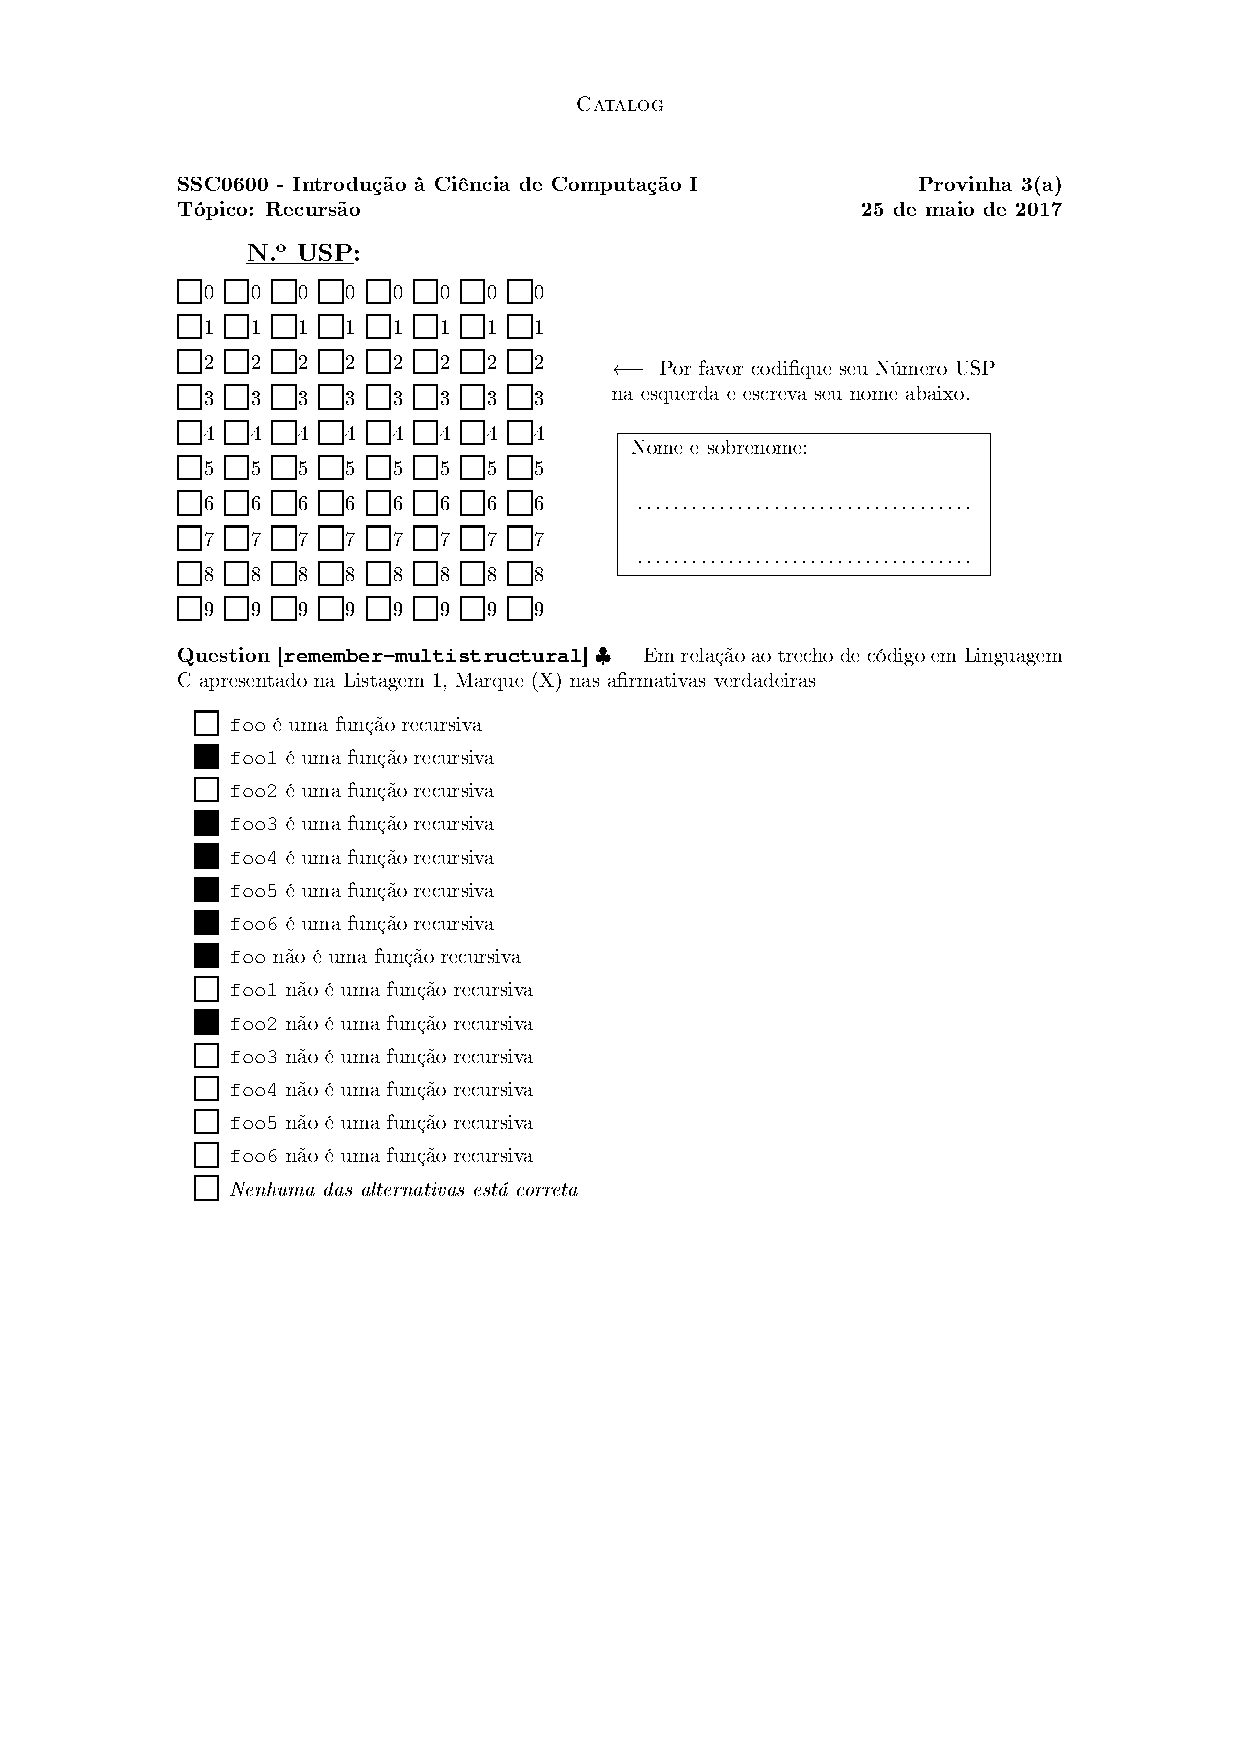
\includegraphics[page=1,width=1\textwidth]{images/annex/third-study-pre.pdf}
\newpage
\includegraphics[page=2,width=1\textwidth]{images/annex/third-study-pre.pdf}
\newpage
\includegraphics[page=3,width=1\textwidth]{images/annex/third-study-pre.pdf}
\newpage
\includegraphics[page=4,width=1\textwidth]{images/annex/third-study-pre.pdf}
\newpage
\includegraphics[page=5,width=1\textwidth]{images/annex/third-study-pre.pdf}
\newpage
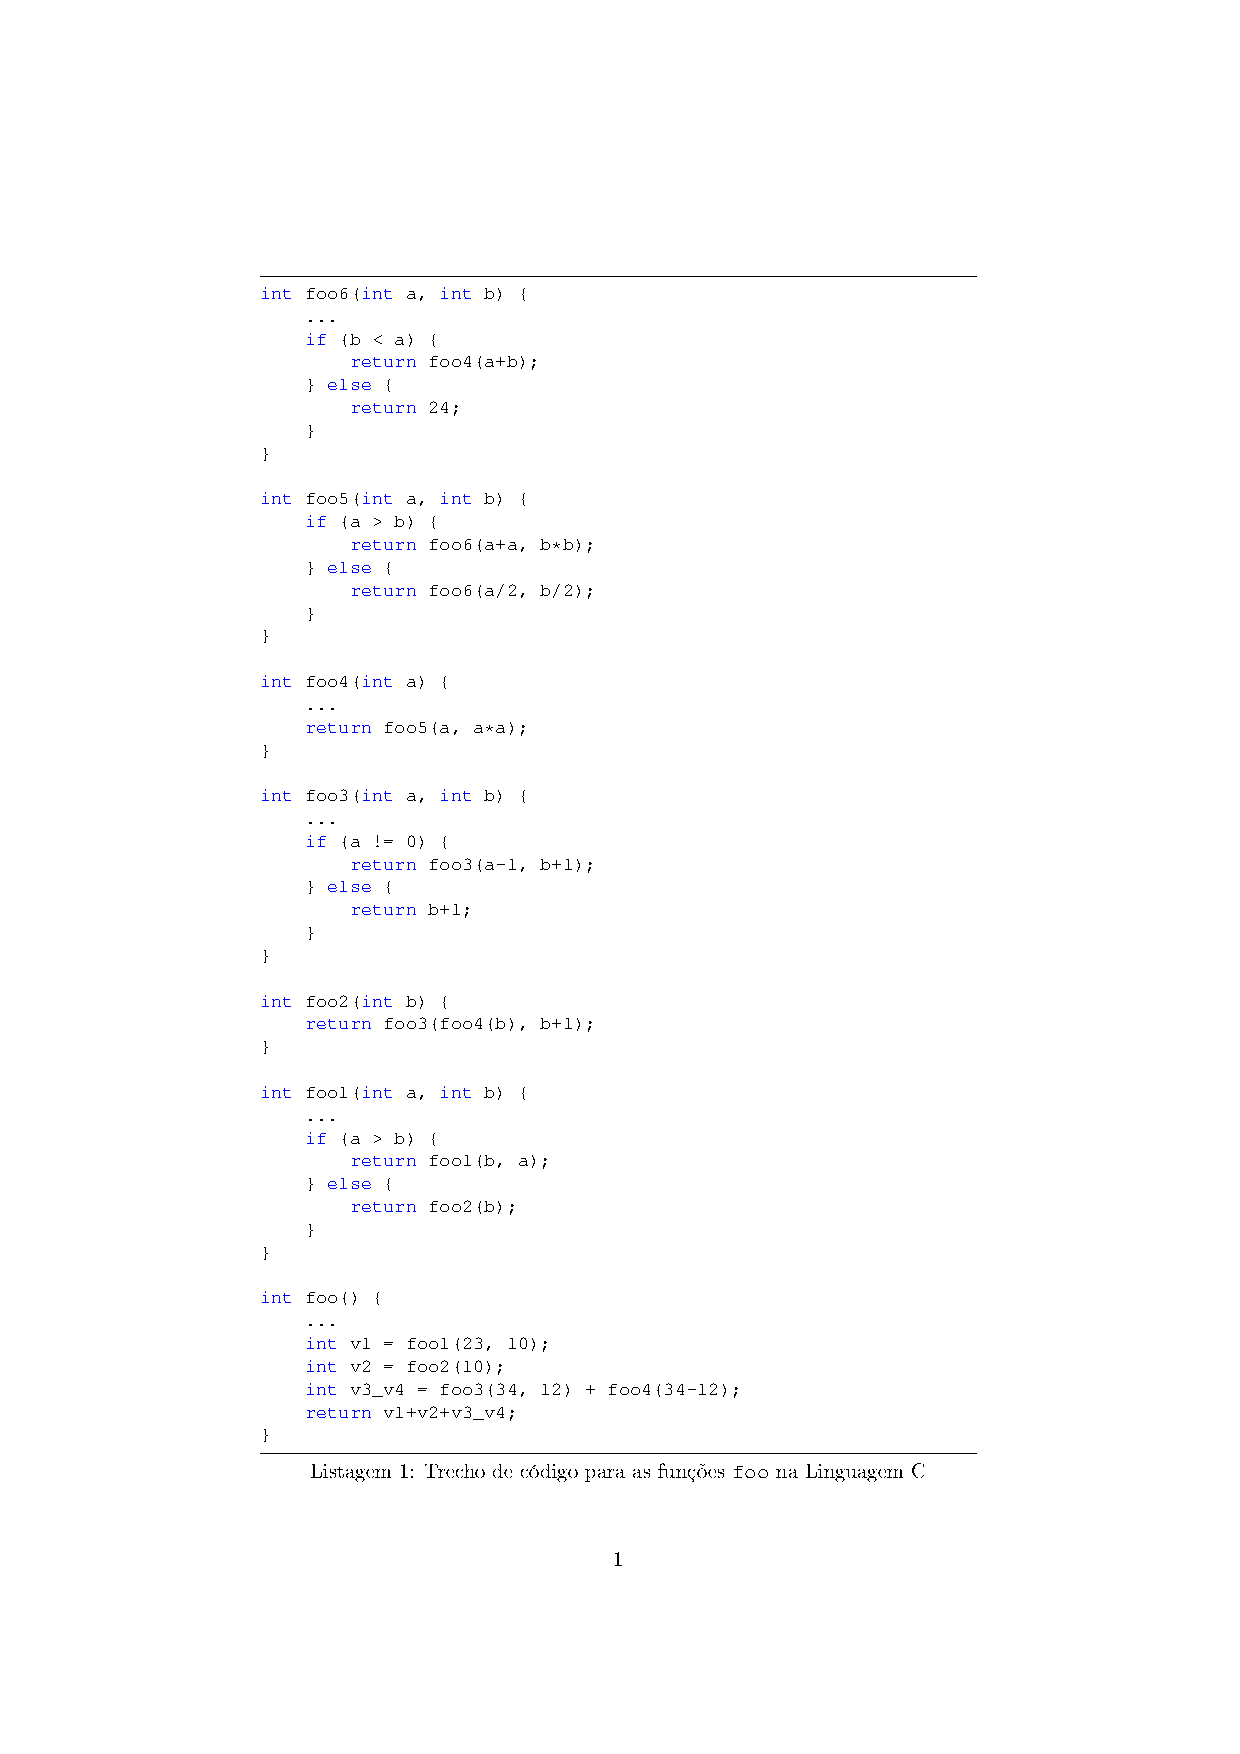
\includegraphics[page=1,width=1\textwidth]{images/annex/third-study-pre-list.pdf}
\newpage
\includegraphics[page=2,width=1\textwidth]{images/annex/third-study-pre-list.pdf}
\newpage
\includegraphics[page=3,width=1\textwidth]{images/annex/third-study-pre-list.pdf}
\newpage
\includegraphics[page=4,width=1\textwidth]{images/annex/third-study-pre-list.pdf}


\newpage
\section{Programming Problem: Calculate Fibonacci Polynomials (P4)}
\label{annex:third-study-p4}
\includegraphics[page=1,width=1\textwidth]{images/annex/third-study-p4.pdf}

%%
\newpage
\section{Formative Evaluation: Multiple Choice Knowledge Questionnaires of Recursion (provinha3c)}
\label{annex:third-study-pos}
\includegraphics[page=1,width=1\textwidth]{images/annex/third-study-pos.pdf}
\newpage
\includegraphics[page=2,width=1\textwidth]{images/annex/third-study-pos.pdf}
\newpage
\includegraphics[page=3,width=1\textwidth]{images/annex/third-study-pos.pdf}
\newpage
\includegraphics[page=4,width=1\textwidth]{images/annex/third-study-pos.pdf}
\newpage
\includegraphics[page=5,width=1\textwidth]{images/annex/third-study-pos.pdf}
\newpage
\includegraphics[page=1,width=1\textwidth]{images/annex/third-study-pos-list.pdf}
\newpage
\includegraphics[page=2,width=1\textwidth]{images/annex/third-study-pos-list.pdf}
\newpage
\includegraphics[page=3,width=1\textwidth]{images/annex/third-study-pos-list.pdf}
\newpage
\includegraphics[page=4,width=1\textwidth]{images/annex/third-study-pos-list.pdf}

\newpage
\section{Programming Problem: Generation of Planning Poker Sequence (PF)}
\label{annex:third-study-pF}
\includegraphics[page=1,width=1\textwidth]{images/annex/third-study-pF.pdf}


\newpage
\section{Programming Problem: Counting Palindromes (PG)}
\label{annex:third-study-pG}
\includegraphics[page=1,width=1\textwidth]{images/annex/third-study-pG.pdf}

\newpage
\section{Programming Problem: Maze Solving Algorithm (PH)}
\label{annex:third-study-pH}
\includegraphics[page=1,width=1\textwidth]{images/annex/third-study-pH.pdf}

%% ========== %%
\chapter{Data Gathering Instruments for Measuring Participants' Motivation}
\label{annex:data-gathering-instruments-motivation}

%\newpage
\section[Web-based Questionnaire for the Adapted Portuguese IMI]{Web-based Questionnaire for the Adapted Portuguese IMI}
\label{annex:IMI-pilot-study}
\includegraphics[width=1\textwidth]{images/annex/IMI-pilot-study.pdf}

\newpage
\section[Paper-based Questionnaire for the Adapted Portuguese IMI]{Paper-based Questionnaire for the Adapted Portuguese IMI}
\label{annex:IMI-first-study}
\includegraphics[width=1\textwidth]{images/annex/IMI-first-study.pdf}

\newpage
\section[Paper-based Questionnaire for the Adapted Portuguese IMMS]{Paper-based Questionnaire for the Adapted Portuguese IMMS}
\label{annex:IMMS-second-study}
\includegraphics[width=1\textwidth]{images/annex/IMMS-second-study.pdf}

\newpage
\section[Web-based Questionnaire for the Adapted Portuguese IMI and IMMS]{Web-based Questionnaire for the Adapted Portuguese IMI and IMMS}
\label{annex:IMI-IMMS-third-study}
\includegraphics[width=1\textwidth]{images/annex/IMI-IMMS-third-study-01.pdf}
\newpage
\includegraphics[width=1\textwidth]{images/annex/IMI-IMMS-third-study-02.pdf}



%% ========== %%


